%% Journal manuscript: stream-function conservative PINN + PoU revision of
%% journal_harry_coupled.tex (kept unchanged). Built from the Elsevier CAS
%% single-column template.

\documentclass[a4paper,fleqn]{cas-sc}

\usepackage[authoryear,longnamesfirst]{natbib}
\shortcites{Rahaman2019}
\usepackage{amsmath,amssymb}
\usepackage{bm}
\usepackage{booktabs}
\usepackage{graphicx}
\usepackage{xcolor}
\usepackage{tikz}
\usetikzlibrary{arrows.meta,calc}
% NOTE: stmaryrd is intentionally NOT loaded. The cas-sc class loads the STIX
% math fonts, which already use all 16 of LaTeX's math symbol-font slots, so
% stmaryrd's \DeclareSymbolFont overflows ("Too many symbol fonts declared").
% STIX provides the same double brackets via \lBrack / \rBrack, used below.

\usepackage{placeins}
\usepackage{float}
\usepackage{capt-of}  % \captionof for non-floating, in-text figures

% Float placement: keep figures near their text and off the end of the paper.
\renewcommand{\topfraction}{0.9}
\renewcommand{\bottomfraction}{0.8}
\renewcommand{\textfraction}{0.07}
\renewcommand{\floatpagefraction}{0.75}

\newcommand{\dd}{\,\mathrm{d}}
\newcommand{\jump}[1]{\lBrack #1 \rBrack}
\newcommand{\Kmat}{\mathbf{K}}
\newcommand{\vflux}{\mathbf{v}}
% Stream-function (curl) reconstruction symbols
\newcommand{\curl}{\nabla\times}          % curl: 3D vector curl; in 2D the out-of-plane convention (d/dy, -d/dx)
\newcommand{\vp}{\vflux_{p}}              % particular field with div vp = f

\newtheorem{theorem}{Theorem}[section]
\newtheorem{lemma}[theorem]{Lemma}
\newtheorem{proposition}[theorem]{Proposition}

\begin{document}
\let\WriteBookmarks\relax
\def\floatpagepagefraction{1}
\def\textpagefraction{.001}

\shorttitle{Locally Conservative CG-LMDFM Flux Reconstruction}
\shortauthors{Harry et al.}

\title[mode=title]{Locally Conservative Flux Reconstruction for Continuous Galerkin Discrete-Fracture Models of Flow and Transport in Fractured Porous Media}

\author[1]{Muchamad Harry Yudha Pratama}
\cormark[1]
\ead{}
\credit{}

\affiliation[1]{organization={Khalifa University of Science and Technology},
            city={Abu Dhabi},
            country={United Arab Emirates}}

\cortext[1]{Corresponding author}

%% ------------------------------------------------------------------
%% TODO (provisional, orange convention): the abstract below is kept
%% verbatim from journal_harry_coupled.tex and still promises the
%% penalty-based NLR-vs-cPINN comparison. It must be rewritten to reflect the
%% current methodology: the hard-curl stream-function construction (conservation
%% by construction), the single-layer fracture generalization (Section 3.2, one
%% network, no penalties, exact on fracture-cut volumes), the PoU sequential
%% update, and the SPE10 coupled study.
%% ------------------------------------------------------------------
\begin{abstract}
Fractured porous media flow simulation demands accurate fracture--matrix coupling and strict local mass conservation. Lagrange multiplier discrete fracture models (LMDFM) represent fractures as codimension-one interfaces with independent fracture and matrix meshes, enforcing pressure continuity weakly. However, standard continuous Galerkin (CG) discretizations are not locally conservative \citep{Koeppel2019}, limiting their use for conservation-law-based flow models. This work develops locally conservative CG FEM formulations for LMDFM in single-phase Darcy flow. Building on an existing methodology \citep{Koeppel2019}, we propose and compare two distinct strategies to restore local conservation of flux in CG formulations, addressing a key limitation of existing approaches. This framework enables direct comparison between accurate element-wise flux reconstruction and physics-informed learning for restoring local conservation. The first strategy extends an existing flux post-processing method for non-fractured domains \citep{DENG2019166} to the LMDFM setting. Locally conservative fluxes are reconstructed on dual mesh interfaces via independent, element-wise local problems. For a triangular element with Lagrange polynomial space of degree-k, the local problem yields a linear system whose size scales with the number of local degrees of freedom. The local solves are fully decoupled, inexpensive, and parallelizable. Fracture interfaces are included in the local balance, yielding locally conservative matrix and fracture fluxes, exact fracture--matrix exchange, and normal-flux continuity across dual mesh interfaces. The second strategy relies on conservative physics-informed neural networks (cPINNs) to locally correct CG fluxes \citep{Jagtap2020}. Unlike standard PINNs, cPINNs employ domain decomposition and enforce local conservation via continuity of normal fluxes across subdomain interfaces, making them well suited for fractured domains. The networks enforce mass balance in the matrix, fractures, and fracture--matrix interfaces using tailored architectures, adaptive activation functions with trainable slopes to accelerate convergence, and training strategies that keep computational cost comparable to element-wise FEM post-processing. Numerical experiments assess both strategies in terms of computational cost, efficiency, and ease of integration with existing FEM solvers. Convergence tests are presented for matrix and fracture pressures and the Lagrange multiplier across several polynomial degrees, validated against academic tests and benchmark cases, including comparison with the TPFA method implemented in MRST. Finally, we illustrate efficient coupling with a saturation transport equation, present preliminary two-phase flow results, and highlight the potential of the proposed approaches for multiphase flow in fractured porous media.
\end{abstract}

\begin{highlights}
\item Placeholder: fracture-aware locally conservative reconstruction for CG-LMDFM fluxes.
\item Placeholder: deterministic and PINN-based reconstructions compared through multiple conservation diagnostics.
\item Placeholder: journal extensions include higher-order tests, fracture-tip/intersection cases, and expanded transport validation.
\end{highlights}

\begin{keywords}
Fractured porous media \sep Continuous Galerkin finite elements \sep Local conservation \sep Flux reconstruction \sep Lagrange multiplier method \sep Saturation transport
\end{keywords}

\maketitle

\section{Introduction}
\label{sec:introduction}

Natural fractures in subsurface formations create high-permeability flow paths that dominate flow in
hydrocarbon reservoirs, geothermal systems, groundwater aquifers, and subsurface storage sites
\citep{Berkowitz2002, Barenblatt1960, WarrenRoot1963, li2008efficient}. Accurately representing fracture--matrix fluid
exchange is therefore essential in reservoir simulation. Discrete fracture--matrix (DFM) models treat
fractures as lower-dimensional interfaces embedded in the rock matrix, explicitly resolving this exchange
\citep{KarimiFard2004}. Conforming DFM methods align the matrix mesh with fracture faces, which becomes
computationally prohibitive for complex fracture networks. Nonconforming approaches (including immersed finite element methods \citep{zhao2024dfm}, embedded
discrete fracture models (EDFM) \citep{Moinfar2014}, and the Lagrange multiplier discrete fracture model
(LMDFM) of \citet{Koeppel2019}) decouple the fracture and matrix meshes. In the LMDFM, pressure continuity across the fracture is enforced weakly, and
the Lagrange multiplier naturally represents the local fracture--matrix exchange flux.

Continuous Galerkin (CG) finite element methods offer practical advantages for fractured-flow simulation:
they support unstructured meshes, standard variational coupling, and separate finite element spaces for
matrix and fracture unknowns. However, standard CG discretizations
do not produce locally conservative fluxes: the net flux through an element's faces does not, in general,
balance the source term within it \citep{DENG2019166}. This is a fundamental limitation for reservoir
simulation, where transport solvers require an elementwise mass balance to advance saturations and
concentrations. Mixed finite element methods based on Raviart--Thomas spaces \citep{raviart2006mixed, brezzi1991mixed}
provide local conservation by construction but at considerably higher implementation cost. Post-processing
strategies offer a practical alternative to this more complex discretization. \citet{cockburn2007} proposed
a two-step postprocessing for standard CG; \citet{DENG2019166} developed an efficient element-wise
reconstruction on nodal dual control volumes for single-phase flow; and \citet{ZHANG201339} applied a
locally conservative Galerkin approach to two-phase flow in porous media. All three post-processing approaches target non-fractured domains and do not account for the exchange
term that couples the matrix and fracture mass balances. Although \citet{ODSAETER2019edfm} construct a
locally conservative flux for embedded fractured-flow discretizations, their formulation is based on a
single continuous pressure field: the fracture--matrix exchange flux is not an explicit degree of freedom
but is instead recovered implicitly through postprocessing. In the LMDFM, the Lagrange multiplier
$\lambda$ directly approximates this exchange flux, making it a natural ingredient for local balance
correction, a property we exploit in the reconstructions developed below.

Physics-informed neural networks (PINNs) \citep{Raissi2019} offer a mesh-agnostic approach to solving
PDEs by embedding governing equations directly in the training loss. \citet{Jagtap2020} extended this framework to domain-decomposed settings, introducing
conservative PINNs (cPINNs) that enforce zero normal-flux jump across subdomain interfaces.
This makes cPINNs a natural starting point for neural network representations
that must capture fracture-induced flux jumps. \citet{Wang2025} applied improved PINNs to fractured-flow simulation using the reinterpreted
discrete fracture model, but local conservation of the flux was not addressed. To our knowledge, locally conservative flux post-processing for CG-based LMDFM formulations has not been systematically studied.

This paper fills this gap by developing and comparing two post-processing strategies for the CG-LMDFM
flux. The first extends the element-wise reconstruction of \citet{DENG2019166} to the fractured LMDFM
setting by incorporating the Lagrange multiplier exchange in the local balance. The second trains a
physics-informed neural network that parameterizes the flux through a stream function, so it is exactly
conservative by construction, and carries the multiplier-driven flux discontinuity across the fracture
through an analytic single-layer field. Several test cases assess local conservation of the reconstructed
flux (a nonfractured manufactured solution, a single-fracture manufactured solution, and the
a sealed boundary-tip fracture case adapted from \citet{Koeppel2019}, including comparison with a MRST/EDFM
reference) and then couple the reconstructed flux to saturation transport, where the stream-function flux
removes the conservation and no-flow-boundary artefacts that the raw CG flux imprints on the saturation
field.
The two strategies are complementary: the numerical reconstruction drives dual-volume residuals to machine
precision, while the PINN approach reduces element-level conservation errors by one to three orders of magnitude;
since it enforces the divergence equation pointwise, this advantage extends beyond element-wise balances
to general control-volume shapes, confirmed by an independent rotated control-volume diagnostic.


\section{Mathematical Model}
\label{sec:model-diagnostics}

We consider a coupled flow and transport problem in a fractured porous medium, in
the hybrid-dimensional setting of the Lagrange-multiplier discrete fracture model
(LMDFM) \citep{Koeppel2019}. The model splits into a pressure problem and a
transport problem for a scalar saturation \(S\), coupled through a
saturation-dependent conductivity. The pressure problem is the total mass
balance---the sum of the phase mass-conservation equations---and sets the total
velocity; the transport problem is the mass-conservation equation of the
transported phase, which advances \(S\). The pressure problem is time-dependent
only through its saturation-dependent coefficient and, in the compressible case,
a storage term, whereas the transport problem carries the genuine time evolution
of the saturation field.
The two are discretized in Section~\ref{sec:flux-reconstruction}, where the
continuous
Galerkin pressure flux is made locally conservative before it drives the
transport.

Let \(\Omega\subset\mathbb{R}^2\) denote the matrix domain and let
\(\Gamma\subset\Omega\) be a lower-dimensional fracture
(Figure~\ref{fig:fracture_schematic}). The matrix pressure is
denoted by \(p\), and the fracture pressure by \(p_\Gamma\). In the Lagrange
multiplier discrete fracture model (LMDFM) \citep{Koeppel2019}, the matrix and
fracture variables may be represented on independent meshes, and pressure
continuity across the fracture is imposed weakly. The multiplier \(\lambda\)
represents the matrix--fracture exchange flux per unit fracture length. It
therefore enters the matrix equation as a concentrated source/sink and the
fracture equation with the opposite sign.

\begin{center}
\centering
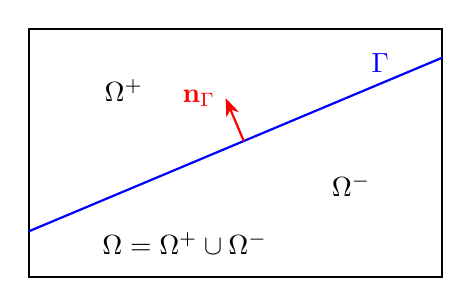
\begin{tikzpicture}[scale=1.05, >=Stealth]
    \draw[thick] (0,0) rectangle (5,3);
    \node at (3,0.15) [anchor=south east] {$\Omega = \Omega^+ \cup \Omega^-$};

    \draw[thick, blue] (0,0.55) -- (5,2.65);
    \node[blue, above] at (4.25,2.35) {$\Gamma$};

    \coordinate (mid) at ($(0,0.55)!0.52!(5,2.65)$);
    \draw[red, ->, thick] (mid) -- ++(-0.22,0.52) node[left] {$\mathbf{n}_\Gamma$};

    \node at (1.15,2.25) {$\Omega^+$};
    \node at (3.9,1.1) {$\Omega^-$};
\end{tikzpicture}
\captionof{figure}{Schematic of a lower-dimensional fracture \(\Gamma\) crossing
the matrix domain \(\Omega\).}
\label{fig:fracture_schematic}
\end{center}

With gravity neglected, the matrix and fracture mass balances, coupled through
\(\lambda\), form the pressure problem, with matrix and fracture
source terms \(f\) and \(f_\Gamma\):
\begin{equation}
\begin{aligned}
c_t\,\partial_t p + \nabla\cdot\left(-\Kmat\nabla p\right) - \lambda \delta_\Gamma &= f
&& \text{in } \Omega,\\
c_{t,\Gamma}\,\partial_t p_\Gamma + \nabla_\Gamma\cdot\left(-\Kmat_\Gamma\nabla_\Gamma p_\Gamma\right) + \lambda &= f_\Gamma
&& \text{on } \Gamma,\\
p|_\Gamma &= p_\Gamma
&& \text{on } \Gamma.
\end{aligned}
\label{eq:lmdfm_strong}
\end{equation}
Here \(\Kmat=\Kmat(S)\) is a saturation-dependent conductivity, a symmetric
positive-definite coefficient that depends on the saturation \(S\) and hence on
time; for brevity we keep the symbol \(\Kmat\) throughout, understanding it to be
evaluated at the current saturation. The coefficient \(c_t\ge 0\) is a storage
coefficient: for \(c_t=0\) the flow is incompressible and the pressure equation is
elliptic at each instant, depending on time only through \(\Kmat(S)\); for \(c_t>0\) the flow is slightly compressible and the pressure
equation is parabolic, carrying its own time derivative. The
saturation enters the pressure problem only through the coefficient \(\Kmat(S)\). When \(c_t=0\) and \(\Kmat\) is
independent of \(S\), the pressure problem decouples and the velocity is frozen.
The fracture conductivity \(\Kmat_\Gamma=\Kmat_\Gamma(S_\Gamma)\) is defined
analogously and includes the fracture aperture, and \(\nabla_\Gamma\) is the
tangential gradient along the fracture. For a straight fracture with unit tangent
\(\bm{\tau}\), \(\nabla_\Gamma p_\Gamma=(\partial_s p_\Gamma)\bm{\tau}\), where
\(s\) is arclength. The term \(\lambda\delta_\Gamma\) denotes a measure
concentrated on the fracture; equivalently,
\[
  \int_\Omega \lambda\delta_\Gamma = \int_\Gamma \lambda .
\]

With \(\vflux=-\Kmat\nabla p\), the multiplier is the jump of the normal Darcy
flux across the fracture \citep{Koeppel2019}. We fix the orientation once and for all: let
\(\Omega^+\) and \(\Omega^-\) denote the two sides of \(\Gamma\), let
\(\mathbf{n}_\Gamma\) be the unit normal pointing from \(\Omega^-\) to
\(\Omega^+\), and for a quantity \(z\) with one-sided traces \(z^\pm\) on
\(\Gamma\) set \(\jump{z}=z^+-z^-\). Explicitly,
\[
  \lambda=\jump{\vflux\cdot\mathbf{n}_\Gamma}
  =-\jump{\Kmat\nabla p\cdot\mathbf{n}_\Gamma}
  \quad \text{on } \Gamma,
\]
that is, writing \(p^+\) and \(p^-\) for the one-sided matrix pressure traces,
\[
  \lambda
  =
  \Kmat\nabla p^-\cdot\mathbf{n}_\Gamma
  -
  \Kmat\nabla p^+\cdot\mathbf{n}_\Gamma .
\]
Thus \(\lambda\) measures the oriented normal-flux imbalance between the two
matrix sides of the fracture.

Let \(V_\Omega\subset H^1(\Omega)\), \(V_\Gamma\subset H^1(\Gamma)\), and
\(\Lambda\subset L^2(\Gamma)\) be the matrix pressure, fracture pressure, and
multiplier spaces. The weak form is: find
\((p,p_\Gamma,\lambda)\in V_\Omega\times V_\Gamma\times\Lambda\) such that, for
all \((q,q_\Gamma,\mu)\in V_\Omega\times V_\Gamma\times\Lambda\),
\begin{equation}
\begin{aligned}
\int_\Omega c_t\,\partial_t p\,q
+\int_\Gamma c_{t,\Gamma}\,\partial_t p_\Gamma\,q_\Gamma
+\int_\Omega \Kmat\nabla p\cdot\nabla q
+\int_\Gamma \Kmat_\Gamma\nabla_\Gamma p_\Gamma\cdot\nabla_\Gamma q_\Gamma
-\int_\Gamma \lambda\left(q|_\Gamma-q_\Gamma\right)
&=
\int_\Omega f q
+\int_\Gamma f_\Gamma q_\Gamma,\\
\int_\Gamma \mu\left(p|_\Gamma-p_\Gamma\right)&=0.
\end{aligned}
\label{eq:lmdfm_weak}
\end{equation}
The first equation is the coupled matrix--fracture mass balance, and the second
enforces pressure continuity across \(\Gamma\) through the multiplier test
functions.

The saturation is advanced by a transport equation in fractional-flow form: the
transported-phase flux is the fractional flow \(F(S)\) times the total velocity
\(\vflux\) \citep{Lie2019}. We assume the fluids are only
slightly compressible, so the compressible accumulation \(c_t\,S\,\partial_t p\)
in the phase balance is small relative to the porosity term \(\phi\,\partial_t S\)
and is neglected; the storage is retained only in the pressure problem (the
\(c_t\,\partial_t p\) and \(c_{t,\Gamma}\,\partial_t p_\Gamma\) terms), where it
keeps the pressure unsteady and sets the time-dependent total velocity that drives
the transport. With porosity \(\phi\) and a source/sink \(q\), the matrix
saturation then satisfies
\begin{equation}
  \phi\,\partial_t S
  + \nabla\cdot\!\left(F(S)\,\vflux\right)
  = q - Q_{m\to\Gamma}
  \quad\text{in }\Omega ,
\label{eq:transport_matrix}
\end{equation}
and the fracture saturation satisfies the one-dimensional analogue
\begin{equation}
  \phi_\Gamma\,\partial_t S_\Gamma
  + \partial_s\!\left(F(S_\Gamma)\,\vflux_\Gamma\cdot\bm\tau\right)
  = q_\Gamma + Q_{m\to\Gamma}
  \quad\text{on }\Gamma ,
\label{eq:transport_fracture}
\end{equation}
where \(\phi_\Gamma\) is the fracture porosity,
\(\vflux_\Gamma=-\Kmat_\Gamma\nabla_\Gamma p_\Gamma\) is the fracture total
velocity, \(s\) is arclength, and \(q_\Gamma\) is the fracture source/sink. The
matrix--fracture exchange of the transported
scalar is the corresponding fraction of the total exchange carried by the
multiplier,
\[
  Q_{m\to\Gamma} = F(S_{\mathrm{up}})\,\lambda ,
\]
with \(S_{\mathrm{up}}\) upwinded according to the sign of the oriented total
exchange \(\lambda\). The system is closed with an initial condition
\(S(\cdot,0)=S_0\) and an inflow condition prescribing \(S\) on the inflow part of
the boundary.

Because the conductivity \(\Kmat(S)\) enters the pressure problem and the total
velocity \(\vflux\) enters the transport problem, the two are coupled both ways:
as the saturation field advances, \(\Kmat(S)\) changes, the pressure field is
updated, and the new velocity advects the saturation further. This coupling is
resolved by the sequential time-stepping algorithm of
Section~\ref{sec:flux-reconstruction}, in which the locally conservative
reconstructed flux drives the transport.

\section{Discretization}
\label{sec:flux-reconstruction}

This section discretizes the model of Section~\ref{sec:model-diagnostics}. The
pressure problem is solved by a continuous Galerkin (CG) LMDFM method, the
transport problem by a standard finite-volume (FV) scheme, and the two are
advanced sequentially in time. Because the CG pressure flux is not locally
conservative, it is post-processed into a conservative flux, by a numerical local
reconstruction (Section~\ref{subsec:nlr}) or a learning-based one
(Section~\ref{subsec:pinn-reconstruction}), before it drives the transport.

We begin with the pressure solve. The continuous Galerkin discretization is
obtained by replacing the continuous
spaces with finite element spaces \(V_{\Omega,h}\), \(V_{\Gamma,h}\), and
\(\Lambda_h\). We seek
\((p_h,p_{\Gamma,h},\lambda_h)\in V_{\Omega,h}\times V_{\Gamma,h}\times
\Lambda_h\) such that, for all
\((q_h,q_{\Gamma,h},\mu_h)\in V_{\Omega,h}\times V_{\Gamma,h}\times\Lambda_h\),
\begin{equation}
\begin{aligned}
\int_\Omega \Kmat\nabla p_h\cdot\nabla q_h
+\int_\Gamma \Kmat_\Gamma\nabla_\Gamma p_{\Gamma,h}\cdot\nabla_\Gamma q_{\Gamma,h}
-\int_\Gamma \lambda_h\left(q_h|_\Gamma-q_{\Gamma,h}\right)
&=
\int_\Omega f q_h
+\int_\Gamma f_\Gamma q_{\Gamma,h},\\
\int_\Gamma \mu_h\left(p_h|_\Gamma-p_{\Gamma,h}\right)&=0.
\end{aligned}
\label{eq:lmdfm_cg}
\end{equation}

Equation~\eqref{eq:lmdfm_cg} is the compact incompressible pressure system,
corresponding to \(c_t=c_{t,\Gamma}=0\) in \eqref{eq:lmdfm_weak}. If
compressible flow is considered, the same CG-LMDFM discretization is used after
adding the storage terms
\(\int_\Omega c_t\,\partial_t p_h\,q_h\) and
\(\int_\Gamma c_{t,\Gamma}\,\partial_t p_{\Gamma,h}\,q_{\Gamma,h}\) to the
left-hand side. With backward Euler at \(t^{n+1}\), these become the mass terms
\((c_t/\Delta t)\int_\Omega p_h^{n+1}\,q_h\) and
\((c_{t,\Gamma}/\Delta t)\int_\Gamma p_{\Gamma,h}^{n+1}\,q_{\Gamma,h}\), with the
previous-time-level contributions moved to the right-hand side.

Because the multiplier \(\lambda_h\) ties the fracture and matrix
pressures together, \eqref{eq:lmdfm_cg} is a saddle-point system whose stability
requires a discrete inf--sup (LBB) condition between the multiplier space
\(\Lambda_h\) and the pressure traces on \(\Gamma\). \citet{Koeppel2019} establish
this condition for the present formulation: it holds when the multiplier mesh
(size \(h_\lambda\)) is kept coarse relative to the matrix mesh (size \(h\)). For a piecewise-constant
multiplier the scheme is stable and convergent provided \(h_\lambda\gtrsim 3h\)
(their Hypothesis~1 and Remark~1), whereas for a continuous piecewise-linear
multiplier a unique solution exists but convergence is not guaranteed; we
therefore keep the multiplier mesh coarse on the nonconforming meshes below.

% Because the multiplier \(\lambda_h\) enters \eqref{eq:lmdfm_cg} as a constraint
% that ties the fracture and matrix pressures together, the system is of
% saddle-point type, and its stability hinges on the multiplier--pressure coupling
% term already present in \eqref{eq:lmdfm_cg},
% \begin{equation}
%   b\big((q_h,q_{\Gamma,h}),\mu_h\big)
%   =\int_\Gamma \mu_h\,(q_h|_\Gamma-q_{\Gamma,h}),
%   \label{eq:bform}
% \end{equation}
% which measures how strongly a trial multiplier \(\mu_h\) acts on the pressure jump
% \(q_h|_\Gamma-q_{\Gamma,h}\) across the fracture. Such a system is well posed only
% when every multiplier is genuinely felt by some pressure pair---the discrete
% inf--sup (or LBB) condition \citep{brezzi1991mixed}: there is a constant
% \(\beta>0\), independent of the mesh, such that
% \begin{equation}
%   \inf_{0\neq\mu_h\in\Lambda_h}\;
%   \sup_{0\neq(q_h,q_{\Gamma,h})\in V_{\Omega,h}\times V_{\Gamma,h}}
%   \frac{b\big((q_h,q_{\Gamma,h}),\mu_h\big)}
%        {\|(q_h,q_{\Gamma,h})\|_{V}\,\|\mu_h\|_{\Lambda}}
%   \;\ge\;\beta,
%   \label{eq:infsup}
% \end{equation}
% with the pressure energy norm
% \(\|(q_h,q_{\Gamma,h})\|_V^2=\int_\Omega|\nabla q_h|^2+\int_\Gamma|\nabla_\Gamma q_{\Gamma,h}|^2\)
% and the mesh-weighted multiplier norm
% \(\|\mu_h\|_\Lambda=h_\lambda^{1/2}\,\|\mu_h\|_{L^2(\Gamma)}\) (the discrete
% \(H^{-1/2}\) norm of \citealp{Koeppel2019}, their Eq.~(20)). In words,
% \eqref{eq:infsup} says that no matter which multiplier one picks, some pressure
% pair responds to it by at least a fixed amount \(\beta\) that does not deteriorate
% as the mesh is refined. This fails when the multiplier space is too rich---its
% mesh too fine relative to the matrix mesh---so that some multiplier modes become
% invisible to the pressure traces, \(\beta\to0\), producing spurious oscillations
% and spoiling convergence.

% \citet{Koeppel2019} establish \eqref{eq:infsup} for the present formulation, with
% the following consequences for our two multiplier choices. For a
% piecewise-constant multiplier \(\beta\) stays bounded below under
% refinement---so the scheme remains stable and convergent---provided the
% multiplier mesh is kept sufficiently coarser than the matrix mesh,
% \(h_\lambda\gtrsim 3h\) (their Hypothesis~1 and Remark~1). For a continuous,
% piecewise-linear multiplier \(\beta\) instead shrinks as the mesh is refined: a
% unique solution still exists, but convergence is no longer guaranteed. This is
% why the nonconforming computations below keep the multiplier mesh coarse.
% Finally, K\"oppel's analysis assumes piecewise-linear (\(k=1\)) pressure; for
% higher-order pressure (\(k\ge 2\)) the compatibility is not separately proved, but
% enriching the pressure space only enlarges the supremum in \eqref{eq:infsup}---
% making the condition easier to satisfy---so stability is expected to persist, and
% we confirm it numerically.

After solving \eqref{eq:lmdfm_cg}, the associated raw matrix CG Darcy flux is
\begin{equation}
  \vflux_h=-\Kmat\nabla p_h .
  \label{eq:raw_cg_flux}
\end{equation}
This flux is accurate, but like standard CG fluxes it is not locally
conservative: it does not satisfy the elementwise mass balance that conservative
transport requires. The reconstruction procedures of the following subsections
therefore take \(\vflux_h\) as their baseline and correct it into a locally
conservative flux. To make this precise, we measure the imbalance on the matrix
mesh \(\mathcal{T}_h\): for an element \(\tau\in\mathcal{T}_h\), define the element
conservation residual
\begin{equation}
R_\tau(\vflux_h,\lambda_h)
=
\int_{\partial\tau}\vflux_h\cdot\mathbf{n}
-
\int_{\tau\cap\Gamma}\lambda_h
-
\int_\tau f .
\label{eq:element_residual}
\end{equation}
This residual measures whether the outward matrix flux over \(\partial\tau\) and
the matrix--fracture exchange inside \(\tau\) balance the matrix source; a flux
with \(R_\tau=0\) for all \(\tau\in\mathcal{T}_h\) is called elementwise locally
conservative. In a time-discrete parabolic solve, the source \(f\) here and in the
local reconstruction below is the effective source
\(f_h^\star=f-c_t(p_h^{n+1}-p_h^n)/\Delta t\); in the incompressible case
\(f_h^\star=f\).

The saturation is advanced by a standard cell-centred upwind finite-volume
discretization of the transport equations
\eqref{eq:transport_matrix}--\eqref{eq:transport_fracture}, locally conservative
by construction. On each face \(e\) of a control volume \(C\), we define the face velocity
\(u_e^n\) from the reconstructed flux \(\widetilde{\vflux}_h^n\)
(Sections~\ref{subsec:nlr}--\ref{subsec:pinn-reconstruction}) and the numerical
transport flux \(j_e^n\) by upwinding the fractional flow,
\[
  u_e^n=\int_e \widetilde{\vflux}_h^n\cdot\mathbf{n}_e,
  \qquad
  j_e^n = F\!\left(S^n_{\mathrm{up},e}\right)u_e^n ,
\]
where \(S^n_{\mathrm{up},e}\) is the saturation of the upstream cell, chosen by the
sign of \(u_e^n\). The matrix--fracture
exchange \(Q_{m\to\Gamma}=F(S^n_{\mathrm{up}})\,\lambda_h^n\) is added to the
fracture cells and subtracted from the cut matrix cells. The explicit update of a
matrix cell is
\begin{equation}
  \phi\,|C|\,\frac{S_C^{n+1}-S_C^n}{\Delta t}
  + \sum_{e\subset\partial C}j_e^n
  = |C|\,q_C^n - Q_C^n ,
  \label{eq:fv_update}
\end{equation}
where
\(Q_C^n=\int_{C\cap\Gamma}\alpha_C^\Gamma\,F(S_{\mathrm{up}}^n)\lambda_h^n\) is the
matrix--fracture exchange assigned to cell \(C\). The weight \(\alpha_C^\Gamma\)
allocates each fracture segment once: \(\alpha_C^\Gamma=1\) when \(\Gamma\) cuts the
interior of \(C\), and \(\alpha_C^\Gamma=1/2\) on each side of a conforming fracture
edge shared by two cells, so that each fracture segment is counted exactly once. The
fracture saturation is advanced by the one-dimensional analogue of this update.
For a fracture control volume \(I_j\),
\[
  \phi_{\Gamma,j}|I_j|
  \frac{S_{\Gamma,j}^{n+1}-S_{\Gamma,j}^{n}}{\Delta t}
  + j_{\Gamma,j+1/2}^{n}-j_{\Gamma,j-1/2}^{n}
  =
  |I_j|q_{\Gamma,j}^{n}+Q_{\Gamma,j}^{n}.
\]
Here \(q_{\Gamma,j}^{n}\) is the cell-averaged fracture source and
\(Q_{\Gamma,j}^{n}=\int_{I_j}F(S_{\mathrm{up}}^n)\lambda_h^n\,\dd s\) is the
exchange received from the matrix. The transported-phase fracture face flux is
\[
  j_{\Gamma,j+1/2}^{n}
  =
  F(S_{\Gamma,\mathrm{up},j+1/2}^{n})\,u_{\Gamma,j+1/2}^{n}.
\]
Unlike the matrix face flux above, which integrates the reconstructed velocity over
the face, the fracture face flux is taken directly from the fracture pressure by a
two-point flux approximation (TPFA): the standard finite-volume flux that
approximates the flux across a face using only the pressures in the two cells
sharing that face (hence \emph{two-point}). Here it is formed from the two adjacent
fracture-pressure values,
\[
  u_{\Gamma,j+1/2}^{n}
  =
  -K_{\Gamma,j+1/2}
  \frac{p_{\Gamma,j+1}^n-p_{\Gamma,j}^n}{\ell_{\Gamma,j+1/2}},
\]
where \(\ell_{\Gamma,j+1/2}\) is the distance between the adjacent fracture
pressure degrees of freedom. This gives directly the single oriented flux per face
that the upwind update needs. The alternative, the element gradient
\(-K_\Gamma\nabla_\Gamma p_{\Gamma,h}\), is a per-segment quantity that would still
have to be reduced to one value per face before it could drive the update; the TPFA
performs that reduction in the standard way, directly from the two adjacent
pressure unknowns. Being
single-valued across faces, this flux lets the fracture transport conserve the
transported saturation; moreover, for piecewise-linear fracture
pressure it also satisfies the discrete fracture mass balance on each cell
(Proposition~\ref{prop:fracture-conservation}, Section~\ref{subsec:fracture-flux}).
We therefore apply the flux reconstruction to the matrix flux
only: the matrix holds the bulk of the transported volume, and its two-dimensional
CG flux is multi-valued across shared element edges, so without reconstruction the
matrix transport would lose mass outright, whereas the one-dimensional fracture
flux is already single-valued and conservative.
A matching reconstruction would be needed only for higher-degree
fracture pressure (Section~\ref{subsec:fracture-flux}); since the transport runs use
\(k=1\), the two-point fracture flux is used as is.

In time, the coupled problem is advanced sequentially. At time level
\(t^n=n\Delta t\) the saturation \(S^n\) is known; we evaluate the conductivity
\(\Kmat(S^n)\), solve \eqref{eq:lmdfm_cg} (or its storage-augmented form above),
obtain \((p_h^n,p_{\Gamma,h}^n,\lambda_h^n)\), reconstruct a locally conservative
total velocity \(\widetilde{\vflux}_h^n\)
(Sections~\ref{subsec:nlr}--\ref{subsec:pinn-reconstruction}), and advance the
saturation to \(S^{n+1}\) by the finite-volume update above. The time step
\(\Delta t\) satisfies the CFL restriction of the explicit transport update. In the
numerical comparisons the transport discretization is kept fixed and only the
velocity supplied to it is changed (either the raw CG flux \(\vflux_h^n\) or a
reconstructed flux \(\widetilde{\vflux}_h^n\)), so differences in the transport
results can be attributed to the flux reconstruction. When \(\Kmat\) is independent
of \(S\), the pressure problem and the reconstruction are computed once and frozen,
recovering a one-way coupled setting.

This pairing (CG for the pressure, FV for the transport) is deliberate: the
pressure and transport equations have different mathematical character, and we
discretize each with the method suited to it. The pressure problem is elliptic:
CG gives high-order accuracy, handles full-tensor conductivity on unstructured
meshes, and provides the variational LMDFM coupling on non-matching fracture and
matrix meshes. The transport problem is hyperbolic: the FV scheme is locally
conservative and upwind-stable at sharp fronts. A pure CG--CG choice would be
unstable at fronts and, being non-conservative, would force a second and
structurally different reconstruction of the transported flux; a pure FV--FV
choice is conservative throughout but gives up the higher-order accuracy and the
variational fracture coupling on the pressure side. We therefore keep CG for the
pressure and FV for the transport, and bridge them by the flux reconstruction
developed next, at the cost of an inexpensive reconstruction step.

The reconstruction itself, developed in the two subsections that follow, retains
the pressure solve \eqref{eq:lmdfm_cg} as the common starting point for all
routes. The objective is not to replace the CG-LMDFM
pressure approximation, but to construct a flux that is compatible with local
mass balance and therefore suitable for conservative transport coupling. We
consider two complementary routes. The first is a deterministic numerical local
reconstruction (NLR), obtained from independent element problems and designed to
enforce balance on nodal dual control volumes. The second is a
PINN-based flux reconstruction, in which the flux is parameterized as a
fixed particular field plus the curl of a learned stream function, so that
local conservation holds by construction on arbitrary control volumes, and
the network is fitted to the raw CG flux. Both methods use the same discrete
multiplier \(\lambda_h\) as the matrix--fracture exchange term.

\subsection{Numerical local reconstruction with fracture exchange}
\label{subsec:nlr}

The deterministic reconstruction extends the continuous Galerkin
post-processing of \citet{DENG2019166} to the LMDFM setting. For each element
\(\tau\), let \(s(\tau,k)\) be the set of local Lagrange degrees of freedom for
polynomial degree \(k\), and let \(\{\phi_\eta\}_{\eta\in s(\tau,k)}\) be the
corresponding nodal basis functions restricted to the element \(\tau\). The
local polynomial space is
\[
  V_h^k(\tau)=\mathrm{span}\{\phi_\eta:\eta\in s(\tau,k)\}.
\]
The element is partitioned into non-overlapping subregions
\(\{t_\xi\}_{\xi\in s(\tau,k)}\), one for each local degree of freedom. The
nodal dual control volume associated with \(\xi\) is denoted by \(C^\xi\);
Figure~\ref{fig:nlr_element_partition} shows this partition for a triangular
element.

\begin{center}
\centering
\includegraphics[width=0.72\linewidth]{figures/element_partition_control_volume.png}
\captionof{figure}{Partition of a triangular element into local control volumes
used in the numerical flux reconstruction.}
\label{fig:nlr_element_partition}
\end{center}

Let \(\psi_\xi\) be the characteristic function of \(t_\xi\), i.e.,
\(\psi_\xi=1\) on \(t_\xi\) and \(\psi_\xi=0\) outside \(t_\xi\). Define the
local interpolation operator
\[
  I_\tau w=\sum_{\xi\in s(\tau,k)} w_\xi \psi_\xi,
  \qquad
  w_\xi=w(\xi).
\]

For an edge or edge segment shared by two neighboring elements \(\tau_1\) and
\(\tau_2\), let \(\{\mathbf{z}\}=(\mathbf{z}|_{\tau_1}+\mathbf{z}|_{\tau_2})/2\)
denote the arithmetic average. The local reconstruction uses
\[
a_\tau(v,w)=\int_\tau \Kmat\nabla v\cdot\nabla w,\qquad
\ell_\tau(w)=\int_\tau f w,
\]
\[
e_\tau(v,w)=\int_{\partial\tau}\{\Kmat\nabla v\}\cdot\mathbf{n}\,w,\qquad
b_\tau(v,w)=\sum_{\xi\in s(\tau,k)}
\int_{\partial C^\xi\cap\partial t_\xi}
(-\Kmat\nabla v\cdot\mathbf{n})\,I_\tau w .
\]
Here \(a_\tau\) is the element stiffness form, \(\ell_\tau\) is the source
functional, \(e_\tau\) transfers boundary-flux information from the CG solution
and neighboring elements, and \(b_\tau\) measures the reconstructed flux through
the local dual-control-volume interfaces.

We first recall the non-fractured reconstruction. Given the CG pressure \(p_h\),
the element-local post-processed pressure
\(\widetilde p_{\tau,h}\in V_h^k(\tau)\) is defined by
\begin{equation}
\begin{aligned}
b_\tau(\widetilde p_{\tau,h},w)
&=
\ell_\tau(I_\tau w-w)
+a_\tau(p_h,w)
+e_\tau(p_h,I_\tau w-w) \qquad \forall w\in V_h^k(\tau).
\end{aligned}
\label{eq:nlr_local_nonfractured}
\end{equation}
Writing
\(\widetilde p_{\tau,h}
=\sum_{\eta\in s(\tau,k)}c_\eta\phi_\eta\), with
\(c_\tau=(c_\eta)_{\eta\in s(\tau,k)}\), gives a small element-local linear
system
\[
  A_\tau c_\tau=\beta_\tau,
\]
where
\[
  (A_\tau)_{\xi\eta}=b_\tau(\phi_\eta,\phi_\xi),
  \qquad
  (\beta_\tau)_\xi
  =
  \ell_\tau(I_\tau\phi_\xi-\phi_\xi)
  +a_\tau(p_h,\phi_\xi)
  +e_\tau(p_h,I_\tau\phi_\xi-\phi_\xi).
\]
Once this local pressure is computed, the reconstructed flux on the element is
obtained by differentiation,
\[
  \widetilde{\vflux}_h|_\tau
  =
  -\Kmat\nabla\widetilde p_{\tau,h} .
\]
Thus the reconstruction does not introduce a new global flux unknown; it solves
one independent element-local problem and then takes the local Darcy gradient.

For fractured elements, the only modification is the lower-dimensional exchange
source carried by the LMDFM multiplier. For a nonconforming fracture, the
segment \(\tau\cap\Gamma\) lies in the interior of the cut element and is
assigned to that element. For a conforming fracture, \(\Gamma\) may lie on an
edge shared by two neighboring elements, so the same geometric segment must be
allocated without double counting. We therefore use fracture-exchange weights
\(\alpha_\tau^\Gamma\): \(\alpha_\tau^\Gamma=1\) on nonconforming
interior cuts, while
\(\alpha_{\tau^+}^\Gamma+\alpha_{\tau^-}^\Gamma=1\) on a conforming fracture
edge shared by \(\tau^+\) and \(\tau^-\). In the conforming case we fix the
equal split \(\alpha_{\tau^+}^\Gamma=\alpha_{\tau^-}^\Gamma=1/2\); no upwinding
is used in this elliptic reconstruction step. This is the same equal-split rule
applied to the matrix--fracture exchange in the transport update
\eqref{eq:fv_update}. With these weights, each fracture
piece is counted once when the element subregions are assembled into a nodal
dual control volume, as made precise in
Lemma~\ref{lem:exchange-consistency}.

We insert this weighted exchange into the element-local reconstruction through
the functional
\begin{equation}
  m_{\tau,h}^\Gamma(w)
  =
  \int_{\tau\cap\Gamma}
  \alpha_\tau^\Gamma \lambda_h\, w .
  \label{eq:nlr_exchange_functional}
\end{equation}
For non-fractured elements \(m_{\tau,h}^\Gamma=0\). The fractured local
reconstruction is then
\begin{equation}
\begin{aligned}
b_\tau(\widetilde p_{\tau,h},w)
&=
\ell_\tau(I_\tau w-w)
+m_{\tau,h}^\Gamma(I_\tau w-w)
+a_\tau(p_h,w)
+e_\tau(p_h,I_\tau w-w), \qquad \forall w\in V_h^k(\tau).
\end{aligned}
\label{eq:nlr_local_problem}
\end{equation}
The fractured local problem uses the same element system matrix \(A_\tau\) as
the non-fractured problem \eqref{eq:nlr_local_nonfractured}, because the
bilinear form \(b_\tau\) is unchanged. Only the right-hand side vector changes,
through the multiplier exchange contribution. The notation covers both
conforming and nonconforming fracture meshes and preserves the total multiplier
exchange over assembled control volumes.

Writing
\(\widetilde p_{\tau,h}=\sum_{\eta\in s(\tau,k)}c_\eta\phi_\eta\) gives a
small element-local linear system
\[
  A_\tau c_\tau=\beta_\tau+\beta_\tau^\Gamma 
\]
where the fracture contribution is
\[
  (\beta_\tau^\Gamma)_\xi
  =
  m_{\tau,h}^\Gamma(I_\tau\phi_\xi-\phi_\xi).
\]
All matrices and right-hand sides are assembled element by element. Hence the
method introduces no additional global solve; the local systems are independent
and can be solved in parallel.

As in the standard NLR post-processing, the local problem
\eqref{eq:nlr_local_problem} is of Neumann type: \(A_\tau\) involves only fluxes,
so adding a constant to the local pressure changes nothing and \(A_\tau\) is
singular, its null space spanned by the constants. Such a system is solvable only
when its right-hand side is balanced: the entries must sum to zero, the discrete
counterpart of requiring zero net source in a pure-flux problem. The exchange
term keeps this balance. The nodal basis and the subregion indicators each form a
partition of unity on \(\tau\) (they sum to one),
\(\sum_{\xi\in s(\tau,k)}\phi_\xi=1\) and
\(\sum_{\xi\in s(\tau,k)}I_\tau\phi_\xi=\sum_{\xi\in s(\tau,k)}\psi_\xi=1\), so by
linearity of \(m_{\tau,h}^\Gamma\),
\[
\sum_{\xi\in s(\tau,k)}
m_{\tau,h}^\Gamma(I_\tau\phi_\xi-\phi_\xi)
=
m_{\tau,h}^\Gamma(1-1)=0,
\]
and the fracture part of the right-hand side sums to zero on its own. The
remaining entries sum to zero by the non-fractured argument
\citep[Lemma~3.1]{DENG2019166}, so the balance condition holds and the singular
local problem stays solvable: the local pressure is fixed only up to an additive
constant (the null space), while its gradient, and hence the reconstructed
flux, is unique.

The reconstructed matrix flux is then
\begin{equation}
  \widetilde{\vflux}_h|_\tau
  =
  -\Kmat\nabla\widetilde p_{\tau,h}.
  \label{eq:nlr_reconstructed_flux}
\end{equation}
Since NLR imposes balance on nodal dual control volumes rather than directly
on elements, we introduce the corresponding diagnostic here. For a node or
degree of freedom \(\xi\) with dual control volume \(C^\xi\), define
\begin{equation}
R_\xi(\mathbf{w},\lambda_h)
=
\int_{\partial C^\xi}\mathbf{w}\cdot\mathbf{n}
-
\int_{C^\xi\cap\Gamma}\lambda_h
-
\int_{C^\xi} f .
\label{eq:dual_residual}
\end{equation}
The fracture integral is absent when \(C^\xi\cap\Gamma=\emptyset\), so the same
definition covers fractured and non-fractured dual volumes.

The construction allocates the fracture exchange to dual volumes without double
counting, which we record before stating the conservation result.

\begin{lemma}[Consistency of the fracture-exchange split]
\label{lem:exchange-consistency}
Let \(C^\xi=\bigcup_{\tau\in\mathcal{T}_\xi}t_\xi^\tau\) be the dual volume of an
interior degree of freedom \(\xi\), and let the exchange weights satisfy
\(\alpha_\tau^\Gamma=1\) on interior nonconforming cuts and
\(\sum_{\tau}\alpha_\tau^\Gamma=1\) on every fracture piece shared by two
elements. Then
\[
\sum_{\tau\in\mathcal{T}_\xi}
\int_{\tau\cap\Gamma}
\alpha_\tau^\Gamma\lambda_h\,I_\tau\phi_\xi
=
\int_{C^\xi\cap\Gamma}\lambda_h .
\]
\end{lemma}

\noindent\emph{Proof.}
On each \(\tau\in\mathcal{T}_\xi\) the local interpolant \(I_\tau\phi_\xi\)
equals the characteristic function \(\psi_\xi\) of the subregion \(t_\xi^\tau\),
so
\[
\int_{\tau\cap\Gamma}\alpha_\tau^\Gamma\lambda_h\,I_\tau\phi_\xi
=
\int_{(t_\xi^\tau)\cap\Gamma}\alpha_\tau^\Gamma\lambda_h .
\]
The subregions \(\{t_\xi^\tau\}_{\tau\in\mathcal{T}_\xi}\) tile \(C^\xi\) without
overlap, and on any fracture piece shared by two of them the weights
\(\alpha_\tau^\Gamma\) sum to one. Summing over \(\mathcal{T}_\xi\) therefore
counts each segment of \(C^\xi\cap\Gamma\) exactly once, which gives
\(\int_{C^\xi\cap\Gamma}\lambda_h\). \(\square\)

\begin{proposition}[Dual-volume conservation]
\label{prop:dual-volume-conservation}
With the fracture-exchange weights of Lemma~\ref{lem:exchange-consistency}, the
NLR flux \(\widetilde{\vflux}_h\) defined by
\eqref{eq:nlr_local_problem}--\eqref{eq:nlr_reconstructed_flux} satisfies
\[
  R_\xi(\widetilde{\vflux}_h,\lambda_h)=0
\]
on every interior nodal dual control volume, up to linear-solver and quadrature
tolerances.
\end{proposition}

\noindent\emph{Proof.}
The local matrix in \eqref{eq:nlr_local_problem} is identical to the
non-fractured problem \eqref{eq:nlr_local_nonfractured}; only the right-hand
side changes by \(m_{\tau,h}^\Gamma\). Accordingly, the argument follows the
structure of the non-fractured post-processing \citep{DENG2019166}, the fracture
exchange being the only new ingredient. Throughout, \(\xi\) is an interior degree
of freedom with element support \(\mathcal{T}_\xi\) and
\(C^\xi=\bigcup_{\tau\in\mathcal{T}_\xi}t_\xi^\tau\).

Test \eqref{eq:nlr_local_problem} with \(w=\phi_\xi|_\tau\) and sum over
\(\mathcal{T}_\xi\). For the left-hand side, recall that the interpolant
\(I_\tau\phi_\xi\) takes the value one on the subregion \(t_\xi^\tau\) and zero
on every other subregion of \(\tau\); hence, in the sum defining \(b_\tau\),
only the interface \(\partial C^\xi\cap\partial t_\xi^\tau\) survives, and
\[
b_\tau(\widetilde p_{\tau,h},\phi_\xi)
=
\int_{\partial C^\xi\cap\partial t_\xi^\tau}
(-\Kmat\nabla\widetilde p_{\tau,h})\cdot\mathbf{n}
=
\int_{\partial C^\xi\cap\partial t_\xi^\tau}
\widetilde{\vflux}_h\cdot\mathbf{n},
\]
the reconstructed normal flux through the part of the dual boundary lying inside
\(\tau\). The subregion boundary \(\partial t_\xi^\tau\) splits as
\(\partial t_\xi^\tau=(\partial\tau\cap\partial t_\xi^\tau)\cup
(\partial C^\xi\cap\partial t_\xi^\tau)\): the element-edge part
\(\partial\tau\cap\partial t_\xi^\tau\) is shared by the subregions of two
adjacent elements and is therefore interior to \(C^\xi\), while the interior
faces \(\partial C^\xi\cap\partial t_\xi^\tau\) assemble across
\(\mathcal{T}_\xi\) to the full dual boundary. Summing therefore gives
\[
\sum_{\tau\in\mathcal{T}_\xi}
b_\tau(\widetilde p_{\tau,h},\phi_\xi)
=
\int_{\partial C^\xi}\widetilde{\vflux}_h\cdot\mathbf{n}.
\]
Turning to the right-hand side, we evaluate the remaining functionals. Using
\(I_\tau\phi_\xi=\psi_\xi\) and \(\bigcup_{\tau}t_\xi^\tau=C^\xi\), the source
functional splits as
\[
\sum_{\tau\in\mathcal{T}_\xi}\ell_\tau(I_\tau\phi_\xi-\phi_\xi)
=
\sum_{\tau\in\mathcal{T}_\xi}\int_{t_\xi^\tau} f
-
\sum_{\tau\in\mathcal{T}_\xi}\int_\tau f\phi_\xi
=
\int_{C^\xi} f-\sum_{\tau\in\mathcal{T}_\xi}\int_\tau f\phi_\xi .
\]
The edge functionals cancel,
\[
\sum_{\tau\in\mathcal{T}_\xi}e_\tau(p_h,I_\tau\phi_\xi-\phi_\xi)=0 ,
\]
because on each interior edge shared by two elements of \(\mathcal{T}_\xi\) the
averaged flux \(\{\Kmat\nabla p_h\}\) is single-valued while the two outward
normals are opposite, so the contributions cancel pairwise, and both
\(\phi_\xi\) and \(I_\tau\phi_\xi\) vanish on the outer boundary of the support.
The average remains single-valued even on a conforming fracture edge, where
\(\Kmat\nabla p_h\) itself jumps by \(\lambda_h\); that jump is carried entirely
by the exchange functional \(m_{\tau,h}^\Gamma\), not by \(e_\tau\). The new
contribution is the fracture exchange: by Lemma~\ref{lem:exchange-consistency},
\[
\sum_{\tau\in\mathcal{T}_\xi}
m_{\tau,h}^\Gamma(I_\tau\phi_\xi-\phi_\xi)
=
\int_{C^\xi\cap\Gamma}\lambda_h
-
\int_\Gamma\lambda_h\phi_\xi ,
\]
while the matrix part of the discrete CG-LMDFM system \eqref{eq:lmdfm_cg},
tested with \((q_h,q_{\Gamma,h},\mu_h)=(\phi_\xi,0,0)\), gives
\[
\sum_{\tau\in\mathcal{T}_\xi}
a_\tau(p_h,\phi_\xi)
-
\int_\Gamma\lambda_h\phi_\xi
=
\sum_{\tau\in\mathcal{T}_\xi}\int_\tau f\phi_\xi .
\]
Substituting this discrete identity into the assembled balance, the auxiliary
terms \(\sum_{\tau}\int_\tau f\phi_\xi\) and
\(\int_\Gamma\lambda_h\phi_\xi\) cancel, leaving
\[
  \int_{\partial C^\xi}\widetilde{\vflux}_h\cdot\mathbf{n}
  =
  \int_{C^\xi}f
  +
  \int_{C^\xi\cap\Gamma}\lambda_h ,
\]
that is, \(R_\xi(\widetilde{\vflux}_h,\lambda_h)=0\). In floating-point
arithmetic the equality holds up to linear-solver and quadrature tolerances.
\(\square\)

The dual-volume identity is algebraic and holds at every step of the coupled
scheme of Section~\ref{subsec:method-coupling}. In the incompressible default
(\(c_t=0\)) the pressure system is exactly \eqref{eq:lmdfm_cg}, with no storage
term. In the parabolic case (\(c_t>0\)), the storage term added to
\eqref{eq:lmdfm_cg} is discretized by backward Euler, and the same proof applies
with the effective-source convention introduced above; no other change is needed.

This property makes NLR a deterministic conservative reference for the
learning-based flux reconstruction. At the same time, because the imposed
balance is the dual-volume balance, the element residual \(R_\tau\) need not be
minimized by this reconstruction.

\subsection{PINN-based reconstruction of CG fluxes}
\label{subsec:pinn-reconstruction}

The learning-based reconstruction also starts from the fixed CG-LMDFM pressure
solution. We reconstruct the matrix flux with a neural network that
represents the flux, rather than the pressure as a standard physics-informed
network would, so the finite element pressure solve is left unchanged and
learning serves only to restore the local conservation of the velocity field.
In physics-informed approaches, the pointwise mass balance is imposed as a
residual term in the training loss \citep{Raissi2019}, enforced only
approximately, with penalty weights to tune; conservative PINNs
\citep{Jagtap2020} add a domain decomposition in which normal-flux continuity
is enforced between the subdomain networks at their interfaces, while the
interior balance still enters as a loss term. The present construction is
instead \emph{conservative by construction}: only exactly conservative fields
are parameterized, so local conservation is a structural property of the
representation and never competes with the data fit during training. The
construction follows the neural-conservation-law principle of
\citet{RichterPowell2022}, built on the classical stream-function
representation of fields with zero divergence.

We first present the construction in the non-fractured base case, where the
matrix domain carries no fracture and the CG flux \(\vflux_h\) of
\eqref{eq:raw_cg_flux} is the only input; the fracture generalization follows
below. The reconstructed flux is the fixed source part plus a correction that the
network supplies,
\begin{equation}
  \vflux_\theta = \vp + \curl\psi_\theta ,
  \label{eq:hardcurl_repr}
\end{equation}
where the network output \(\psi_\theta\) is a stream function: a three-component
field in three dimensions, and a single scalar in two. In three dimensions
\(\curl\psi_\theta\) is the ordinary curl of a vector field; in two dimensions
\(\psi_\theta\) is read as the single out-of-plane component, so that
\(\curl\psi_\theta=(\partial\psi_\theta/\partial y,\,
-\partial\psi_\theta/\partial x)\). In both cases \(\vp\) is a fixed
\emph{particular field} satisfying \(\nabla\cdot\vp=f\), constructed from \(f\)
once, before training; it carries the entire source budget, does not depend on
\(\theta\), and is recomputed only when \(f\) changes. Because
\(\nabla\cdot(\curl\psi_\theta)=0\) in both dimensions, the representation
\eqref{eq:hardcurl_repr} satisfies \(\nabla\cdot\vflux_\theta=\nabla\cdot\vp=f\)
\emph{identically}, whatever the network parameters. Local conservation on
arbitrary control volumes is then immediate.

\begin{proposition}[Conservation by construction on arbitrary control volumes]
\label{prop:hardcurl-conservation}
Let \(\vflux_\theta\) be the reconstruction \eqref{eq:hardcurl_repr} with
\(\nabla\cdot\vp=f\) and the network output \(\psi_\theta\) of class
\(C^1(\overline\Omega)\) (a scalar in two dimensions, a three-component field in
three). Then for every control volume \(\omega\subseteq\Omega\) with Lipschitz
boundary,
\[
  R_\omega(\vflux_\theta)
  =
  \int_{\partial\omega}\vflux_\theta\cdot\mathbf{n}
  -
  \int_\omega f
  =
  0
\]
in exact arithmetic.
\end{proposition}

\noindent\emph{Proof.}
The correction in \eqref{eq:hardcurl_repr} is a curl, whose divergence vanishes,
so \(\nabla\cdot\vflux_\theta=\nabla\cdot\vp=f\) pointwise in \(\Omega\); the
divergence theorem on \(\omega\) then gives
\(\int_{\partial\omega}\vflux_\theta\cdot\mathbf{n}
=\int_\omega\nabla\cdot\vflux_\theta
=\int_\omega f\). \(\square\)

In contrast with the NLR identity of
Proposition~\ref{prop:dual-volume-conservation}, which holds on the designed
nodal dual volumes, Proposition~\ref{prop:hardcurl-conservation} holds on
\emph{any} control volume \(\omega\) (element, dual volume, rotated volume, or
boundary volume), with no reference to the mesh that produced \(\vflux_h\).

Proposition~\ref{prop:hardcurl-conservation} holds at the continuous level,
balancing the exact boundary integral
\(\int_{\partial\omega}\vflux_\theta\cdot\mathbf{n}\) against \(\int_\omega f\).
In a discrete computation this boundary integral is usually approximated by
quadrature, whose error would leave a nonzero residual and break the
machine-precision balance. That error never arises here. In two dimensions the face
fluxes of the curl part are exact endpoint differences of \(\psi_\theta\): for a
straight face \(e\) running from endpoint \(\mathbf{a}\) to endpoint
\(\mathbf{b}\), with
unit tangent \(\bm\tau\) and normal \(\mathbf{n}\) obtained by rotating
\(\bm\tau\) clockwise, \((\curl\psi)\cdot\mathbf{n}=\partial\psi/\partial\tau\)
along \(e\), so
\begin{equation}
  \int_e \vflux_\theta\cdot\mathbf{n}
  =
  \psi_\theta(\mathbf{b})-\psi_\theta(\mathbf{a})
  +
  \int_e \vp\cdot\mathbf{n} ,
  \label{eq:hardcurl_face_flux}
\end{equation}
with the \(\vp\) integral precomputed once per face. Summing
\eqref{eq:hardcurl_face_flux} over the faces of any closed control-volume
boundary, the endpoint values of \(\psi_\theta\) telescope to zero. The
reconstruction (the curl part) therefore contributes exactly nothing to the
control-volume balance, for any coefficients and independent of quadrature, and
so can never break conservation; the only quadrature that remains is that of the
fixed particular-field flux \(\int_e\vp\cdot\mathbf{n}\), a one-time term
independent of the reconstruction. In three dimensions the same exactness holds by
Stokes' theorem: the flux of \(\nabla\times\psi_\theta\) through a flat face
equals the loop integral of \(\psi_\theta\) along the face edges, and these
edge integrals cancel in pairs around any closed control volume, so the correction
again adds exactly nothing, independent of quadrature.

The same face identity lets a no-flow (homogeneous Neumann) boundary be enforced
exactly, rather than through a penalty. Let \(\Sigma\subset\partial\Omega\) be a
connected boundary segment on which \(\vflux\cdot\mathbf{n}=0\) is required,
parametrized by arclength \(s\in[0,|\Sigma|]\) with unit tangent \(\bm\tau\) and
outward normal \(\mathbf{n}\). Along the boundary the curl part contributes the
tangential derivative of the stream function,
\((\curl\psi_\theta)\cdot\mathbf{n}=\partial\psi_\theta/\partial\tau\), so on any
sub-segment \((s_1,s_2)\subset\Sigma\) the reconstructed flux integrates to
\[
  \int_{s_1}^{s_2}\vflux_\theta\cdot\mathbf{n}\,\dd s
  =
  \bigl[\psi_\theta(s_2)-\psi_\theta(s_1)\bigr]
  +\int_{s_1}^{s_2}\vp\cdot\mathbf{n}\,\dd s .
\]
Requiring the right-hand side to vanish for \emph{every} sub-segment determines
the boundary trace of \(\psi_\theta\) up to a single additive constant,
\begin{equation}
  \psi_\theta\bigl(\mathbf{x}(s)\bigr)
  = c_\Sigma-\int_0^{s}\vp\cdot\mathbf{n}\,\dd s',
  \qquad s\in[0,|\Sigma|].
  \label{eq:noflow_trace}
\end{equation}
The integrand is known before training, so \eqref{eq:noflow_trace} is a
one-dimensional antiderivative of the fixed-field normal flux, evaluated in
closed form and imposed as a hard constraint on the boundary trace of
\(\psi_\theta\). Because \eqref{eq:noflow_trace} holds for every \(s\), the
integrand itself vanishes:
\(\vflux_\theta\cdot\mathbf{n}
=\partial\psi_\theta/\partial\tau+\vp\cdot\mathbf{n}=0\) pointwise on
\(\Sigma\), for any network parameters and independently of quadrature, by
the same endpoint-difference identity that yields the conservation property,
now read along the boundary. Each connected no-flow segment carries its own
constant \(c_\Sigma\); only differences of the trace within a segment enter any
flux, so the constants are immaterial. When \(\vp\cdot\mathbf{n}\equiv0\) on
\(\Sigma\), the trace \eqref{eq:noflow_trace} reduces to a constant, the
classical statement that an impermeable boundary is a streamline.

The network and its training are shaped by the heterogeneous fields the stream
function must represent. \(\psi_\theta\) is a fully connected multilayer
perceptron with a smooth activation, so that the flux \(\curl\psi_\theta\) is
well defined pointwise. Its input is a Fourier-feature embedding of the
coordinates, which counteracts the spectral bias of coordinate networks in
highly heterogeneous media \citep{Tancik2020,WangWang2021}, augmented by a
log-permeability feature \(\log\kappa(\mathbf{x})\) that informs the network
of the local coefficient scale. The architecture and training settings are
reported with the numerical studies. Training is plain data fitting: the loss matches the reconstructed flux to the CG
flux \(\vflux_h\) through two terms, both least-squares misfits of the same
solution, an integrated face-flux term over the dual faces and a pointwise
flux-sample term, weighted by \(w_{\mathrm f}\) and \(w_{\mathrm p}\),
\begin{equation}
  \mathcal{L}(\theta)
  =
  w_{\mathrm f}\sum_{e\in\mathcal{E}_h^{\mathrm{dual}}}
  \Bigl(\int_e\left(\vflux_\theta-\vflux_h\right)\cdot\mathbf{n}\Bigr)^2
  +
  w_{\mathrm p}\sum_{\mathbf{x}_j\in\mathcal{X}}
  \bigl\|\vflux_\theta(\mathbf{x}_j)-\vflux_h(\mathbf{x}_j)\bigr\|^2 ,
  \label{eq:hardcurl_loss}
\end{equation}
where \(\mathcal{E}_h^{\mathrm{dual}}\) collects the dual-mesh faces,
\(\mathcal{X}\) a fixed set of sample points, and
\(w_{\mathrm f},w_{\mathrm p}\ge0\) the two term weights. The first term uses the integrated
dual-face fluxes; by the decomposition \eqref{eq:hardcurl_face_flux} each of its
summands is evaluated in closed form,
\[
  \int_e\left(\vflux_\theta-\vflux_h\right)\cdot\mathbf{n}
  =
  \psi_\theta(\mathbf{b}_e)-\psi_\theta(\mathbf{a}_e)
  +\int_e\vp\cdot\mathbf{n}
  -\int_e\vflux_h\cdot\mathbf{n} ,
\]
its only network evaluations being point values of \(\psi_\theta\) at the face
endpoints \(\mathbf{a}_e,\mathbf{b}_e\), the two integrals precomputed. The second
term uses the local flux values \(\vflux_h(\mathbf{x}_j)\). The two carry
complementary information about the same \(\vflux_h\), and their relative effect on
accuracy is examined in Section~\ref{subsec:single-fracture-benchmark}; the
settings are reported with the numerical studies.

Neither term is a conservation penalty, because none is needed: where a
penalty-based physics-informed loss balances a data term against a
divergence term through tuned weights, here the entire conservation budget is
carried by the representation \eqref{eq:hardcurl_repr}, and training only
distributes the accuracy information of \(\vflux_h\). A poorly trained network
is therefore inaccurate but still exactly conservative; training error affects
accuracy, never mass balance.

We now generalize the construction to fractured domains. Across the physical
fracture network \(\Gamma=\cup_{\ell=1}^{N_\Gamma}\Gamma_\ell\) the matrix flux is
discontinuous: its normal component jumps by the matrix--fracture exchange, which
in the LMDFM is the discrete multiplier \(\lambda_h\), known once the CG solve is
complete (Section~\ref{sec:model-diagnostics}).

We carry this jump analytically, through the particular field. To \(\vp\) we add a
fracture field \(\vflux_{p,\lambda}\) whose normal component jumps by exactly
\(\lambda_h\) as one crosses \(\Gamma\). We build it by placing sources of strength
\(\lambda_h\) along the fracture and adding up the field each one produces. A single
unit source at \(\mathbf{x}'\in\Gamma\) has potential
\(G(\mathbf{x},\mathbf{x}')=-\tfrac{1}{2\pi}\log\|\mathbf{x}-\mathbf{x}'\|\) for
\(d=2\) and \(\tfrac{1}{4\pi\|\mathbf{x}-\mathbf{x}'\|}\) for \(d=3\)
\citep[\S2.2]{Evans2010}. Summing over \(\Gamma\) gives the potential and its field,
\begin{equation}
  u_\lambda(\mathbf{x})
  =
  \int_{\Gamma}
  G(\mathbf{x},\mathbf{x}')\,\lambda_h(\mathbf{x}')\,\mathrm{d}s(\mathbf{x}') ,
  \qquad
  \vflux_{p,\lambda}
  =
  -\nabla u_\lambda ,
  \qquad
  \mathbf{x}\in\Omega,\ \mathbf{x}'\in\Gamma ,
  \label{eq:single_layer_field}
\end{equation}
the single-layer potential of \(\lambda_h\). The one property we use is the
following.

\begin{lemma}[The single-layer field carries the fracture exchange]
\label{lem:single_layer}
Let \(\Gamma\) be a codimension-one interface in \(\Omega\subseteq\mathbb{R}^d\),
\(d\in\{2,3\}\) (a curve in two dimensions, a surface in three), with unit normal
\(\mathbf{n}_\Gamma\), and let \(\vflux_{p,\lambda}=-\nabla u_\lambda\)
with \(u_\lambda\) from \eqref{eq:single_layer_field}. Then
\(\nabla\cdot\vflux_{p,\lambda}=0\) in \(\Omega\setminus\Gamma\), its normal
component jumps across \(\Gamma\) by
\(\jump{\vflux_{p,\lambda}\cdot\mathbf{n}_\Gamma}=\lambda_h\), and for every control
volume \(\omega\),
\[
  \int_{\partial\omega}\vflux_{p,\lambda}\cdot\mathbf{n}
  =
  \int_{\Gamma\cap\omega}\lambda_h .
\]
\end{lemma}

\noindent\emph{Proof.} The only tools are the divergence theorem, the interchange
of two integrals, and the one property of the point source, that it obeys
\(-\Delta G(\mathbf{x},\mathbf{x}')=\delta(\mathbf{x}-\mathbf{x}')\)
\citep[\S2.2]{Evans2010}, so that its outward flux over any region equals \(1\)
when the source point lies inside and \(0\) when it lies outside. Take first a
point \(\mathbf{x}\notin\Gamma\); then \(\mathbf{x}\neq\mathbf{x}'\) for every
\(\mathbf{x}'\in\Gamma\), so \(G(\mathbf{x},\mathbf{x}')\) is smooth in
\(\mathbf{x}\) and we may differentiate \(u_\lambda\) under the integral sign, and
since each \(G(\cdot,\mathbf{x}')\) solves Laplace's equation away from its source
point (in polar coordinates about \(\mathbf{x}'\), \(\Delta G=0\) for
\(\mathbf{x}\neq\mathbf{x}'\)),
\[
  \Delta u_\lambda(\mathbf{x})
  =
  \int_\Gamma \Delta G(\mathbf{x},\mathbf{x}')\,\lambda_h(\mathbf{x}')=0 ,
  \qquad \mathbf{x}\notin\Gamma ,
\]
so \(\nabla\cdot\vflux_{p,\lambda}=-\Delta u_\lambda=0\) off the fracture.

For the balance on a control volume \(\omega\), write
\(\vflux_{p,\lambda}=-\nabla u_\lambda\) and differentiate under the integral,
\[
  \int_{\partial\omega}\vflux_{p,\lambda}\cdot\mathbf{n}
  =
  -\int_{\partial\omega}\!\int_\Gamma
  \nabla G(\mathbf{x},\mathbf{x}')\cdot\mathbf{n}(\mathbf{x})\,
  \lambda_h(\mathbf{x}') .
\]
Interchanging the two integrals and, for each fixed source point \(\mathbf{x}'\),
applying the divergence theorem on \(\omega\),
\[
  \int_{\partial\omega}
  \nabla G(\mathbf{x},\mathbf{x}')\cdot\mathbf{n}(\mathbf{x})
  =
  \int_\omega \Delta G(\mathbf{x},\mathbf{x}')
  =
  \begin{cases}
    -1, & \mathbf{x}'\in\omega,\\[2pt]
    \phantom{-}0, & \mathbf{x}'\notin\omega,
  \end{cases}
\]
by the point-source property. Interchanging the order and inserting this value,
\[
  \int_{\partial\omega}\vflux_{p,\lambda}\cdot\mathbf{n}
  =
  -\int_\Gamma\!\Bigl(\int_{\partial\omega}
  \nabla G(\mathbf{x},\mathbf{x}')\cdot\mathbf{n}\Bigr)\lambda_h
  =
  -\int_{\Gamma\cap\omega}(-1)\,\lambda_h
  =
  \int_{\Gamma\cap\omega}\lambda_h ,
\]
since the inner integral is \(-1\) for \(\mathbf{x}'\in\Gamma\cap\omega\) and \(0\)
otherwise. This is the stated balance.

The normal jump follows by applying the balance to a thin box across the fracture.
Take \(\omega\) to be a slab of thickness \(2\varepsilon\) straddling the fracture,
and let \(S=\Gamma\cap\omega\) be the piece of \(\Gamma\) inside it; the slab has
one face on each side of \(\Gamma\) and thin walls joining them. As
\(\varepsilon\to0\) the walls carry no flux and the two faces collapse onto
\(S\), with outward normal \(+\mathbf{n}_\Gamma\) on the plus side and
\(-\mathbf{n}_\Gamma\) on the minus side, so the balance
\(\int_{\partial\omega}\vflux_{p,\lambda}\cdot\mathbf{n}=\int_S\lambda_h\) becomes
\[
  \int_S\bigl(\vflux_{p,\lambda}^{+}-\vflux_{p,\lambda}^{-}\bigr)\cdot\mathbf{n}_\Gamma
  =\int_S\lambda_h .
\]
As \(S\) is arbitrary, the integrands agree pointwise,
\(\jump{\vflux_{p,\lambda}\cdot\mathbf{n}_\Gamma}=\lambda_h\). \(\square\)

\smallskip\noindent
In shorthand, the two facts just shown read
\(\nabla\cdot\vflux_{p,\lambda}=\lambda_h\,\delta_\Gamma\): no source off
\(\Gamma\), source \(\lambda_h\) on it.

The sign is chosen so that \(\lambda_h\) acts as a source in the matrix, matching
the CG-LMDFM system. Because the interface is codimension one, the lemma covers a
surface fracture in a three-dimensional matrix without change, using the
three-dimensional \(G\) above. The jump is thus carried by this analytic term,
computed once from the known \(\lambda_h\) before any training.

The reconstructed flux uses a single stream function over the whole matrix
domain,
\begin{equation}
  \vflux_\theta
  =
  \vflux_{p,f} + \vflux_{p,\lambda} + \curl\psi_\theta ,
  \label{eq:hardcurl_fractured_flux}
\end{equation}
where \(\vflux_{p,f}\) is the source particular field of the base case
(\(\nabla\cdot\vflux_{p,f}=f\)) and \(\psi_\theta\) is one smooth network as
before. The three parts split the mass balance cleanly: \(\vflux_{p,f}\) supplies
the source \(f\), \(\vflux_{p,\lambda}\) supplies the fracture exchange on
\(\Gamma\) (Lemma~\ref{lem:single_layer}), and the curl term supplies neither,
since \(\nabla\cdot(\curl\psi_\theta)=0\). So on any control volume \(\omega\),
\begin{equation}
  \int_{\partial\omega}\vflux_\theta\cdot\mathbf{n}
  =
  \int_\omega f
  +
  \int_{\Gamma\cap\omega}\lambda_h .
  \label{eq:hardcurl_fracture_balance}
\end{equation}
This is the fracture-aware form of
Proposition~\ref{prop:hardcurl-conservation}: the boundary flux of every control
volume balances its interior source plus the exchange it receives from the
fracture pieces crossing it. Fracture-cut volumes are included, and the balance
holds to machine precision, because the analytic field carries the jump exactly
while, as in \eqref{eq:hardcurl_face_flux}, the curl part's face fluxes sum to
zero around any closed control-volume boundary. The only integral that still needs
quadrature is the one-time particular-field face flux
\(\int_e(\vflux_{p,f}+\vflux_{p,\lambda})\cdot\mathbf{n}\), and for a straight
fracture with the piecewise multiplier of the CG solve, the fracture part of it is
available in closed form.

Training is unchanged from the non-fractured case: the same flux-fitting loss
\eqref{eq:hardcurl_loss}, now with the particular field
\(\vflux_{p,f}+\vflux_{p,\lambda}\). The fracture physics lives entirely in that
fixed analytic field, so a poorly trained network is inaccurate but still exactly
conservative on every control volume, fracture-cut ones included.

The construction extends to a fracture network by superposition. Each branch
\(\Gamma_\ell\) contributes its own single-layer term from its multiplier
\(\lambda_{h,\ell}\), and these add,
\begin{equation}
  \vflux_{p,\lambda}=\sum_{\ell=1}^{N_\Gamma}\vflux_{p,\lambda_\ell} ,
  \label{eq:multi_fracture_source}
\end{equation}
so the jump relation holds on each branch separately and the balance
\eqref{eq:hardcurl_fracture_balance} becomes
\(\int_{\partial\omega}\vflux_\theta\cdot\mathbf{n}
=\int_\omega f+\sum_\ell\int_{\Gamma_\ell\cap\omega}\lambda_{h,\ell}\),
exact on every control volume, including volumes cut by several fractures or
containing an intersection: the densities superpose linearly, and the mass
balance at an intersection is the one the CG multiplier system already encodes.
Adding a fracture adds a term to a sum; the single network and the penalty-free
training are unchanged.

\subsubsection{Sequential flux updates by a partition of unity}
\label{subsubsec:pou-head}

In the coupled time-dependent problem of Section~\ref{subsec:method-coupling},
the flux must be reconstructed every time the saturation is updated, that is, at
every transport step, once the pressure has been re-solved. An efficient way to
update the reconstruction across these steps is therefore needed, and is the aim
of this subsubsection. Because the target flux changes little from
one step to the next, and what change there is stays confined to a moving
neighbourhood of the saturation front, each reconstruction is naturally
obtained by updating the network trained at the previous step rather than
training a new one from scratch. In the trained network, the stream function is
produced by a \emph{final linear layer}: the weighted sum
\(\psi=\mathbf{h}(\mathbf{x})^{\!\top}\mathbf{w}\), where
\(\mathbf{h}(\mathbf{x})\in\mathbb{R}^{W}\) is the last hidden layer's output
vector (\(W\) the layer width) and \(\mathbf{w}\) holds the coefficients.

Given this structure (nonlinear hidden layers feeding a linear final
layer), there are several natural ways to refresh the reconstruction from the
previous step's network, differing in whether they re-fit the features
\(\mathbf{h}(\mathbf{x})\), the coefficients \(\mathbf{w}\), or both. One may
(i) re-optimize the whole network or (ii) re-optimize only part of it; both
change the features \(\mathbf{h}(\mathbf{x})\), on which the network depends
nonlinearly, so each step is a nonlinear optimization (Adam, or L-BFGS).
Alternatively, (iii) keep the features \(\mathbf{h}(\mathbf{x})\) fixed and
re-fit only the coefficients \(\mathbf{w}\) by least squares against the new CG
face fluxes. This is very fast, requiring only the solution of one linear
system, but its accuracy against the new CG flux is not guaranteed: with the
features frozen, the update is limited to a linear re-weighting of them, which
need not reproduce a target flux that has changed nonlinearly, and a single
\(\mathbf{w}\) shared over the whole domain applies that re-weighting uniformly
everywhere. A fourth option, (iv), the one we develop, keeps the closed-form cost of (iii)
but replaces the single global \(\mathbf{w}\) by a \emph{localized} set of
coefficients that can adjust the reconstruction differently near the front and
away from it.

To make the coefficients local, we give different parts of the domain their own
coefficient vectors. On its own, this would make the reconstruction jump at the
boundaries between parts; to keep it a single smooth field, the local pieces are
combined through smoothly overlapping weights that form a \emph{partition of
unity}, a way of blending local approximations into a single global one
\citep{MelenkBabuska1996}. These weights are built as follows. We cover the
domain by \(N_w\) overlapping \emph{windows} on a regular grid: each window is a
smooth weight function \(\chi_k\), largest at its centre and falling to zero at
its edge, built as a smooth profile along \(x\) multiplied by the same profile
along \(y\). The windows are made somewhat larger than the grid spacing so that
neighbours overlap, so a typical point of the domain lies inside two to four
windows at once, and we normalize them, dividing each by their pointwise sum,
so that at every point of the domain they add up to one. This normalized
family \(\{\chi_k\}\) is the partition of unity introduced above. The same
device, in neural-network settings, has also been explored in the random
feature method and partition-of-unity networks
\citep{ChenRFM2022,LeeTrask2021}. Two consequences matter here. First, because
the weights sum to one, giving every window the same coefficients collapses the
blend to a single global linear layer: the partition-of-unity layer generalizes
the ordinary final linear layer and can always fall back to it, so the
partition by itself distorts nothing. Second, the normalized weights remain
continuously differentiable, which is essential because the flux is a
derivative of the stream function.
Figure~\ref{fig:pou_windows} illustrates these weights in one dimension.

\begin{center}
\centering
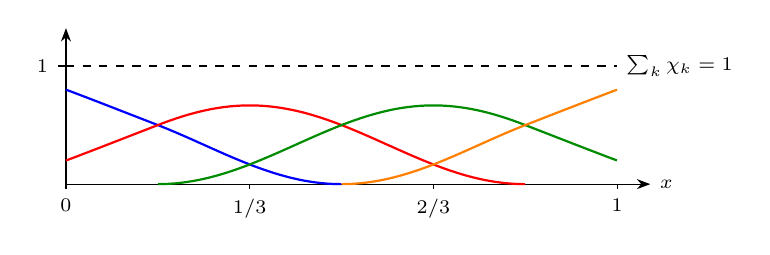
\begin{tikzpicture}[x=7cm,y=1.5cm,>=Stealth]
  \pgfmathdeclarefunction{pouwin}{2}{%
    \pgfmathparse{(abs(#1-#2)<0.5)*(cos(180*(#1-#2)))^2}%
  }
  \pgfmathdeclarefunction{pousum}{1}{%
    \pgfmathparse{pouwin(#1,0)+pouwin(#1,0.33333)+pouwin(#1,0.66667)+pouwin(#1,1)}%
  }
  \draw[->] (0,0) -- (1.06,0) node[right,font=\scriptsize] {$x$};
  \draw[->] (0,0) -- (0,1.32);
  \foreach \xc/\lab in {0/{$0$},0.33333/{$1/3$},0.66667/{$2/3$},1/{$1$}}
    \draw (\xc,0) -- (\xc,-0.04) node[below,font=\scriptsize] {\lab};
  \draw[dashed] (0,1) -- (1,1) node[right,font=\scriptsize] {$\textstyle\sum_k\chi_k=1$};
  \draw (0,1) -- (-0.015,1) node[left,font=\scriptsize] {$1$};
  \draw[blue,thick,          domain=0:0.5,      samples=60] plot (\x,{pouwin(\x,0)/pousum(\x)});
  \draw[red,thick,           domain=0:0.83333,  samples=80] plot (\x,{pouwin(\x,0.33333)/pousum(\x)});
  \draw[green!55!black,thick,domain=0.16667:1,  samples=80] plot (\x,{pouwin(\x,0.66667)/pousum(\x)});
  \draw[orange,thick,        domain=0.5:1,      samples=60] plot (\x,{pouwin(\x,1)/pousum(\x)});
\end{tikzpicture}
\captionof{figure}{The partition of unity in one dimension: four overlapping
windows \(\chi_k\) (centres at \(0,\tfrac13,\tfrac23,1\)), normalized so that at
every point of the domain they add up to one (dashed line); blending the
windows' predictions with these weights then introduces no distortion of its
own.}
\label{fig:pou_windows}
\end{center}

We use this partition of unity to replace the trained network's final linear
layer: in place of the single global combination
\(\psi=\mathbf{h}(\mathbf{x})^{\!\top}\mathbf{w}\), each window carries its own
coefficient vector, and the stream function is their windowed blend,
\begin{equation}
  \psi(\mathbf{x})
  =
  \sum_{k=1}^{N_w}
  \chi_k(\mathbf{x})\,
  \mathbf{h}(\mathbf{x})^{\!\top}\mathbf{w}_k ,
  \label{eq:pou_head}
\end{equation}
where \(\mathbf{w}_k\in\mathbb{R}^{W}\) is the coefficient vector of window
\(k\) (the local counterpart of the single global \(\mathbf{w}\), acting on the
same hidden features \(\mathbf{h}(\mathbf{x})\)), so that at each point the
stream function is the \(\chi_k\)-weighted average of the predictions
\(\mathbf{h}(\mathbf{x})^{\!\top}\mathbf{w}_k\) of the windows that cover the
point. Concretely, each window \(\chi_k\) is the squared cosine
\(\widetilde\chi(t)=\cos^2(\pi t/2)\) on \(|t|\le1\) and zero outside, formed in
each coordinate as \(\widetilde\chi\bigl((x-c_k)/s\bigr)\) with \(c_k\) the
window centre and \(s\) its half-width, multiplied across the two coordinates
and then divided by the pointwise sum of all such weights so that
\(\sum_k\chi_k\equiv1\). The squared cosine reaches zero with vanishing slope at
\(|t|=1\), so each compactly supported window is \(C^1\) (the smoothness the
flux needs, being a derivative of \(\psi\)), and overlapping squared-cosine
windows are a standard partition-of-unity choice in domain-decomposed networks
\citep{Moseley2023}.

To keep the per-step solve small, each window's coefficients are restricted to
a common \(r\)-dimensional subspace, \(\mathbf{w}_k=P\theta_k\) with
\(\theta_k\in\mathbb{R}^{r}\) and \(r\ll W\), where the columns of
\(P\in\mathbb{R}^{W\times r}\) are the trained \(\mathbf{w}\) together with the
\(r-1\) leading principal directions of the hidden features, obtained by a
principal component analysis (PCA) of \(\mathbf{h}\) sampled at the collocation
points, i.e.\ the directions along which the features vary most across the
domain.
Each window then carries only \(r\) coefficients \(\theta_k\) instead of the
full \(W\). Its prediction can be written as
\(\mathbf{h}(\mathbf{x})^{\!\top}\mathbf{w}_k
=\mathbf{h}(\mathbf{x})^{\!\top}P\theta_k
=\left(P^{\top}\mathbf{h}(\mathbf{x})\right)^{\!\top}\theta_k\), which is an
\(r\)-dimensional linear combination, with coefficients \(\theta_k\), of the
fixed projected features \(P^{\top}\mathbf{h}(\mathbf{x})\).
Because the original trained coefficient vector \(\mathbf{w}\) is included as
one of the columns of \(P\), it belongs to the reduced subspace
\(\operatorname{span}(P)\). Hence there exists a coefficient vector
\(\theta^{(0)}\in\mathbb{R}^r\) such that \(P\theta^{(0)}=\mathbf{w}\).
Therefore, every window can choose \(\theta_k=\theta^{(0)}\), giving
\(\mathbf{w}_k=P\theta_k=\mathbf{w}\) exactly. The sequential updates are
therefore \emph{warm-started} from this trained solution (begun from an initial
guess that is already close, rather than from scratch), so each step need only
apply a small correction. Figure~\ref{fig:pou_pipeline} summarizes how the
frozen features feed the window coefficients.

\begin{center}
\centering
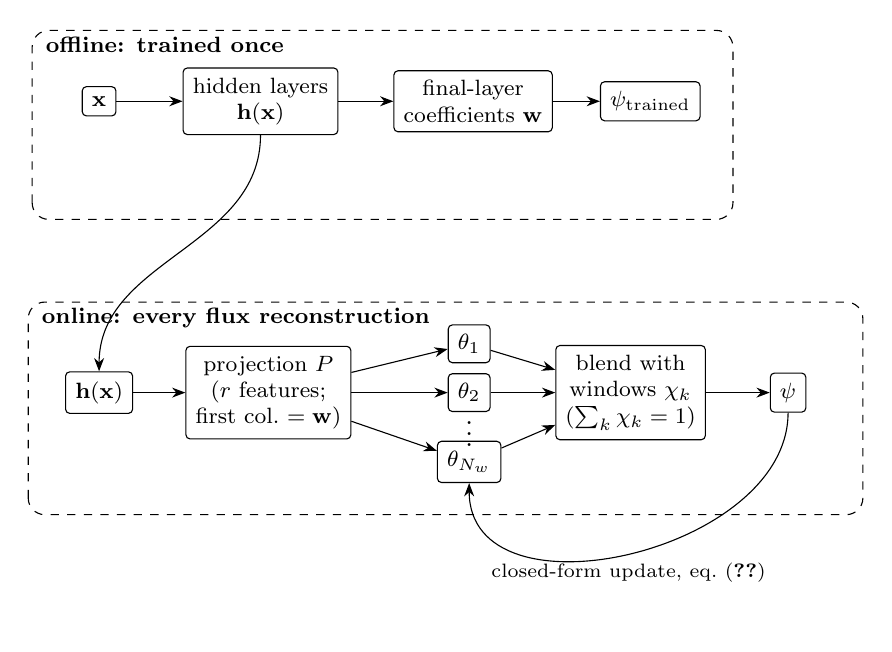
\begin{tikzpicture}[>=Stealth,
  box/.style={draw,rounded corners=1.5pt,align=center,font=\footnotesize,inner sep=3.5pt},
  ann/.style={font=\scriptsize\itshape,align=center}]
  % ---- offline group ----
  \node[box] (x1)   at (0,0)   {$\mathbf{x}$};
  \node[box] (h1)   at (2.05,0) {hidden layers\\ $\mathbf{h}(\mathbf{x})$};
  \node[box] (w1)   at (4.75,0) {final-layer\\ coefficients $\mathbf{w}$};
  \node[box] (psi1) at (7.0,0)  {$\psi_{\mathrm{trained}}$};
  \draw[->] (x1)--(h1); \draw[->] (h1)--(w1); \draw[->] (w1)--(psi1);
  % \node[ann] at (3.4,-1.05) {hidden features frozen after training};
  \draw[dashed,rounded corners=6pt] (-0.85,-1.5) rectangle (8.05,0.9);
  \node[font=\footnotesize\bfseries,anchor=west] at (-0.8,0.72)
    {offline: trained once};
  % ---- online group ----
  \begin{scope}[yshift=-3.7cm]
    \node[box] (h2)    at (0,0)    {$\mathbf{h}(\mathbf{x})$};
    \node[box] (P2)    at (2.15,0) {projection $P$\\ ($r$ features;\\ first col.\ $=\mathbf{w}$)};
    \node[box] (t1)    at (4.7,0.62) {$\theta_1$};
    \node[box] (t2)    at (4.7,0.0)  {$\theta_2$};
    \node       (td)   at (4.7,-0.42) {$\vdots$};
    \node[box] (tn)    at (4.7,-0.88) {$\theta_{N_w}$};
    \node[box] (bl)    at (6.75,0)  {blend with\\ windows $\chi_k$\\ ($\sum_k\chi_k=1$)};
    \node[box] (psi2)  at (8.75,0)  {$\psi$};
    \draw[->] (h2)--(P2);
    \draw[->] (P2)--(t1); \draw[->] (P2)--(t2); \draw[->] (P2)--(tn);
    \draw[->] (t1)--(bl); \draw[->] (t2)--(bl); \draw[->] (tn)--(bl);
    \draw[->] (bl)--(psi2);
    \draw[dashed,rounded corners=6pt] (-0.9,-1.55) rectangle (9.7,1.15);
    \node[font=\footnotesize\bfseries,anchor=west] at (-0.85,0.95)
      {online: every flux reconstruction};
  \end{scope}
  % ---- cross links ----
  \draw[->] (h1.south) to[out=-90,in=90]
    node[midway,left,font=\scriptsize,align=center] { } (h2.north);
  \draw[->] (psi2.south) to[out=-90,in=-90,looseness=1.1]
    node[midway,below,font=\scriptsize] {closed-form update, eq.~\eqref{eq:pou_update}} (tn.south);
\end{tikzpicture}
\captionof{figure}{The two-stage pipeline. Offline (top), the network is
trained once; its hidden features \(\mathbf{h}(\mathbf{x})\) and final-layer
coefficients \(\mathbf{w}\) are then frozen. Online (bottom), the frozen features are
reused: a fixed projection \(P\) reduces them to \(r\) combinations (the first
being the trained one), each window carries its own coefficient vector
\(\theta_k\), and the window predictions are blended by the partition of
unity into the stream function \(\psi\). Only the \(\theta_k\) are recomputed
at each step, by the closed-form update \eqref{eq:pou_update}.}
\label{fig:pou_pipeline}
\end{center}

We next describe how these window coefficients enter the flux update. Consider
one window \(k\). It carries \(r\) coefficients in the form of \(\theta_k\), and its
contribution to any dual face's flux is linear in these coefficients. Indeed,
by \eqref{eq:hardcurl_face_flux}, the flux through a dual face \(e\), oriented
from endpoint \(\mathbf{a}_e\) to \(\mathbf{b}_e\), is obtained by differencing
the stream function \(\psi\) between the two endpoints, up to the fixed
particular-field flux. Since, by \eqref{eq:pou_head}, the dependence of
\(\psi\) on \(\theta_k\) enters only through the fixed window \(\chi_k\) and the
fixed features \(\mathbf{h}\), window \(k\)'s contribution to face \(e\) can be
written as \(\mathbf{g}_{e,k}^{\top}\theta_k\), where
\[
  \mathbf{g}_{e,k}
  =
  P^{\top}\bigl[\chi_k(\mathbf{b}_e)\,\mathbf{h}(\mathbf{b}_e)
  -\chi_k(\mathbf{a}_e)\,\mathbf{h}(\mathbf{a}_e)\bigr]\in\mathbb{R}^{r}.
\]
Thus, \(\mathbf{g}_{e,k}\) is the \(\chi_k\)-weighted difference of the projected
features between the two endpoints of the face. If window \(k\) were updated on
its own, its coefficients would follow from a small \(r\)-dimensional
least-squares fit of these flux contributions to the new CG face fluxes.

The windows are coupled, however: where they overlap, one face's flux draws on
several windows' coefficients at once, so all windows are fitted together.
Writing, for each dual face \(e\),
\[
  F_{h,e}=\int_e \vflux_h\cdot\mathbf{n}_e\,\dd s,
  \qquad
  F_{\vp,e}=\int_e \vp\cdot\mathbf{n}_e\,\dd s,
\]
for the integrated normal flux of the new CG solution and of the fixed
particular field, and collecting these over the \(M\) dual faces into
\(F_{h},F_{\vp}\in\mathbb{R}^{M}\), the window coefficients
\(\theta=(\theta_1,\ldots,\theta_{N_w})\) are fitted by
\begin{equation*}
\underbrace{\begin{pmatrix}
\mathbf{g}_{e_1,1}^{\top} & \mathbf{g}_{e_1,2}^{\top} & \cdots & \mathbf{g}_{e_1,N_w}^{\top}\\[2pt]
\mathbf{g}_{e_2,1}^{\top} & \mathbf{g}_{e_2,2}^{\top} & \cdots & \mathbf{g}_{e_2,N_w}^{\top}\\
\vdots & \vdots & & \vdots\\
\mathbf{g}_{e_M,1}^{\top} & \mathbf{g}_{e_M,2}^{\top} & \cdots & \mathbf{g}_{e_M,N_w}^{\top}
\end{pmatrix}}_{\Phi\,\in\,\mathbb{R}^{M\times N_w r}}
\underbrace{\begin{pmatrix}\theta_1\\ \theta_2\\ \vdots\\ \theta_{N_w}\end{pmatrix}}_{\theta}
\;\approx\;
\underbrace{\begin{pmatrix}
F_{h,e_1}-F_{\vp,e_1}\\
F_{h,e_2}-F_{\vp,e_2}\\
\vdots\\
F_{h,e_M}-F_{\vp,e_M}
\end{pmatrix}}_{F_{h}-F_{\vp}}
\end{equation*}
Each row corresponds to one dual face and holds one block per window; by the
support of the windows, \(\mathbf{g}_{e,k}\) vanishes for every window \(k\) that
contains neither endpoint of face \(e\), so at most two to four of the \(N_w\)
blocks in a row are nonzero. A face lying inside a single window constrains only
that window's coefficients; a face in an overlap ties its windows together. This
coupling is what makes the fit global, while the few nonzero blocks per row
leave \(\Phi\) sparse. The update minimizes the face-flux misfit plus a
regularization,
\[
  \min_{\theta}\;
  \bigl\|\Phi\theta-(F_{h}-F_{\vp})\bigr\|^2
  +\rho\,\bigl\|\theta-\theta_{\mathrm{anchor}}\bigr\|^2 .
\]
The second term, with weight \(\rho>0\), is a \emph{ridge} (Tikhonov)
regularization that does two jobs: it keeps the normal matrix well conditioned,
and it holds that window's coefficients at their previous values
\(\theta_{\mathrm{anchor}}\) instead of letting them drift. The minimizer solves
the normal equations
\begin{equation}
  \left(\Phi^{\top}\Phi+\rho I\right)\theta
  =
  \Phi^{\top}\!\left(F_{h}-F_{\vp}\right)
  +\rho\,\theta_{\mathrm{anchor}} .
  \label{eq:pou_update}
\end{equation}
The geometry, windows, and features never change, so the matrix \(\Phi\) and the
normal matrix \(\Phi^{\top}\Phi+\rho I\) are assembled and factorized a single
time (cheaply, since the sparsity of \(\Phi\) makes \(\Phi^{\top}\Phi\) sparse
too), and each refresh afterwards costs only a pair of triangular solves. Conservation is preserved at every update: the blended
\(\psi\) of \eqref{eq:pou_head} is a single-valued \(C^1\) scalar field for any
coefficients, so Proposition~\ref{prop:hardcurl-conservation} and the
telescoping of \eqref{eq:hardcurl_face_flux} hold unchanged at every step. The
particular field \(\vp\) is reused across refreshes as long as \(f\) is
unchanged; only the window coefficients move.

Two stages thus divide the labour. Offline, the network is trained once by
minimizing the least-squares flux-fitting loss \eqref{eq:hardcurl_loss}, which
fixes the features \(\mathbf{h}\) and the projection \(P\). Online, within the coupled simulation,
where the evolving saturation changes the pressure, and hence the target CG
flux, from one step to the next, only the window coefficients are refreshed, by
the closed-form solve above. This is option~(iv) of the update strategies set
out at the start of this subsubsection: each refresh is a single linear solve,
as in the global linear fit~(iii) but localized so it can track the moving
front, and far cheaper than the per-step nonlinear optimization of~(i) and~(ii). 
\subsection{Local conservation of the fracture flux}
\label{subsec:fracture-flux}

Both matrix-flux reconstructions of the previous subsections, the deterministic
NLR (Section~\ref{subsec:nlr}) and the PINN
(Section~\ref{subsec:pinn-reconstruction}), act on the two-dimensional matrix
flux; the one-dimensional fracture flux is common to both. Here we fix that
fracture flux, establish its local conservation under the assumptions set out
below (\(P_1\) fracture pressure, \(P_0\) source and multiplier), and then
explain why, in that case, an element-local reconstruction is not needed for it.

The fracture transport update consumes one tangential flux per face of the fracture
mesh, and two quantities are available from the CG-LMDFM fracture pressure
\(p_{\Gamma,h}\). The first is the finite-element element-gradient flux
\[
  \vflux_{\Gamma,h}=-K_\Gamma\,\partial_s p_{\Gamma,h},
\]
a per-element field, constant on each element for $P_1$ pressure. The
second is the two-point (TPFA) face flux between adjacent nodes \(j\) and \(j+1\),
\[
  u_{\Gamma,j+1/2}=-K_{\Gamma,j+1/2}\,
  \frac{p_{\Gamma,j+1}-p_{\Gamma,j}}{\ell_{\Gamma,j+1/2}},
\]
with \(K_{\Gamma,j+1/2}/\ell_{\Gamma,j+1/2}\) the transmissibility of the element
between nodes \(j\) and \(j+1\), of length \(\ell_{\Gamma,j+1/2}=x_{j+1}-x_j\) and
conductivity \(K_{\Gamma,j+1/2}\). The half-integer index marks the inter-nodal
element and the face at its midpoint, so node \(j\) is flanked by elements of lengths
\(\ell_{\Gamma,j-1/2}\) and \(\ell_{\Gamma,j+1/2}\). For $P_1$ pressure the
element gradient
on \([x_j,x_{j+1}]\) is exactly
\(-K_\Gamma(p_{\Gamma,j+1}-p_{\Gamma,j})/\ell_{\Gamma,j+1/2}\), so the two definitions
coincide on every face; they differ only for higher-degree pressure
(\(P_2\) and above), where \(\vflux_{\Gamma,h}\) carries the interior polynomial
modes while \(u_{\Gamma,j+1/2}\) uses the endpoint values alone. Being single-valued per face, the two-point flux is the one the
transport update uses.

\begin{center}
\centering
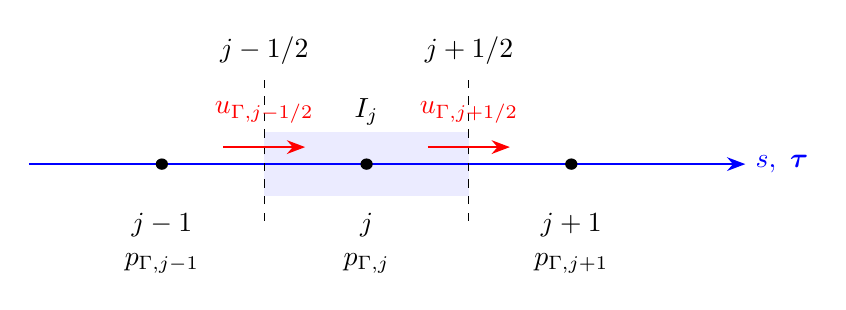
\begin{tikzpicture}[>=Stealth,x=1.3cm,y=1.2cm]
  \color{black}% keep the diagram black inside the orange block
  % node-centred control volume I_j (the dual cell)
  \fill[blue!8] (-1,-0.34) rectangle (1,0.34);
  % fracture line, arclength s / tangent tau
  \draw[thick,blue] (-3.3,0) -- (3.0,0);
  \draw[->,thick,blue] (3.0,0) -- (3.7,0) node[right] {$s,\ \bm\tau$};
  % faces (dual-cell boundaries) at the element midpoints
  \draw[dashed] (-1,-0.6) -- (-1,0.95);
  \draw[dashed] ( 1,-0.6) -- ( 1,0.95);
  \node[above] at (-1,0.95) {$j-1/2$};
  \node[above] at ( 1,0.95) {$j+1/2$};
  % nodes (fracture-pressure DOFs)
  \fill (-2,0) circle (0.06);
  \fill ( 0,0) circle (0.06);
  \fill ( 2,0) circle (0.06);
  \node[below,align=center] at (-2,-0.42) {$j-1$\\$p_{\Gamma,j-1}$};
  \node[below,align=center] at ( 0,-0.42) {$j$\\$p_{\Gamma,j}$};
  \node[below,align=center] at ( 2,-0.42) {$j+1$\\$p_{\Gamma,j+1}$};
  % two-point face fluxes (positive in +s)
  \draw[->,thick,red] (-1.4,0.18) -- (-0.6,0.18);
  \draw[->,thick,red] ( 0.6,0.18) -- ( 1.4,0.18);
  \node[red] at (-1,0.55) {$u_{\Gamma,j-1/2}$};
  \node[red] at ( 1,0.55) {$u_{\Gamma,j+1/2}$};
  % cell name
  \node at (0,0.55) {$I_j$};
\end{tikzpicture}
\captionof{figure}{One-dimensional fracture stencil. The node-centred control volume
\(I_j\) (shaded) spans the two faces \(j\mp1/2\) at the midpoints of the elements
adjoining node \(j\). The two-point face fluxes \(u_{\Gamma,j\mp1/2}\) (red), each
formed from the two adjacent nodal pressures \(p_{\Gamma,\bullet}\).}
\label{fig:fracture_stencil}
\end{center}

The local-conservation requirement is the one-dimensional analogue of the element
residual \eqref{eq:element_residual}: integrating the fracture pressure equation
\eqref{eq:lmdfm_strong} over the node-centred control volume \(I_j\) of node \(j\)
(the interval between the midpoints of the two adjacent elements;
Figure~\ref{fig:fracture_stencil}) gives
\begin{equation}
\int_{\partial I_j}\vflux_{\Gamma,h}\cdot\bm\tau
=
\int_{I_j} f_\Gamma - \int_{I_j}\lambda_h ,
\label{eq:fracture_balance}
\end{equation}
the net tangential outflow balancing the fracture source and the matrix--fracture
exchange (with the effective source of Section~\ref{subsec:nlr} in the parabolic
case). The two-point flux supplies the boundary term as
\(\int_{\partial I_j}\vflux_{\Gamma,h}\cdot\bm\tau=u_{\Gamma,j+1/2}-u_{\Gamma,j-1/2}\),
so local conservation reduces to the following.

\begin{proposition}[Local conservation of the CG fracture flux]
\label{prop:fracture-conservation}
Let the fracture pressure be \(P_1\) with nodal hat basis
\(\{\phi_{\Gamma,j}\}\), and let \(f_\Gamma\) and \(\lambda_h\) be \(P_0\)
on the fracture mesh. Then on every interior fracture node \(j\),
\[
  u_{\Gamma,j+1/2}-u_{\Gamma,j-1/2}
  =
  \int_\Gamma\bigl(f_\Gamma-\lambda_h\bigr)\,\phi_{\Gamma,j}\,\dd s .
\]
Hence the two-point fracture flux is locally conservative on every interior cell
\(I_j\).
\end{proposition}

\noindent\emph{Proof.}
Test the discrete system \eqref{eq:lmdfm_cg} with
\((q_h,q_{\Gamma,h},\mu_h)=(0,\phi_{\Gamma,j},0)\). The terms in \(q_h\) drop and the
coupling term gives \(-\int_\Gamma\lambda_h(0-\phi_{\Gamma,j})\), leaving
\[
  \int_\Gamma K_\Gamma\,\partial_s p_{\Gamma,h}\,\partial_s\phi_{\Gamma,j}
  +\int_\Gamma\lambda_h\,\phi_{\Gamma,j}
  =\int_\Gamma f_\Gamma\,\phi_{\Gamma,j}.
\]
The hat \(\phi_{\Gamma,j}\) is supported on the two elements adjacent to node \(j\):
on the left element \([x_{j-1},x_j]\) of length \(\ell_{\Gamma,j-1/2}\) its slope is
\(\partial_s\phi_{\Gamma,j}=+1/\ell_{\Gamma,j-1/2}\), and on the right element
\([x_j,x_{j+1}]\) of length \(\ell_{\Gamma,j+1/2}\) it is \(-1/\ell_{\Gamma,j+1/2}\).
Evaluate the conductivity at the two faces, \(K_{\Gamma,j-1/2}\) and
\(K_{\Gamma,j+1/2}\) and
recall that \(\partial_s p_{\Gamma,h}\) is the constant element slope of the
\(P_1\) pressure. The contribution of each element is then
\(K_{\Gamma,j\mp1/2}\) times the product of the two constant slopes times the element
length, and the length cancels the \(1/\ell\) carried by the basis slope, leaving
exactly one two-point face flux per element,
\[
  \int_{x_{j-1}}^{x_j} K_\Gamma\,\partial_s p_{\Gamma,h}\,\partial_s\phi_{\Gamma,j}
  =K_{\Gamma,j-1/2}\,\frac{p_{\Gamma,j}-p_{\Gamma,j-1}}{\ell_{\Gamma,j-1/2}}
  =-\,u_{\Gamma,j-1/2},
\]
\[
  \int_{x_j}^{x_{j+1}} K_\Gamma\,\partial_s p_{\Gamma,h}\,\partial_s\phi_{\Gamma,j}
  =-\,K_{\Gamma,j+1/2}\,\frac{p_{\Gamma,j+1}-p_{\Gamma,j}}{\ell_{\Gamma,j+1/2}}
  =u_{\Gamma,j+1/2}.
\]
Since \(\phi_{\Gamma,j}\) vanishes outside these two elements,
\(\int_\Gamma=\int_{x_{j-1}}^{x_j}+\int_{x_j}^{x_{j+1}}\), so adding the two lines
gives
\[
  \int_\Gamma K_\Gamma\,\partial_s p_{\Gamma,h}\,\partial_s\phi_{\Gamma,j}
  =u_{\Gamma,j+1/2}-u_{\Gamma,j-1/2},
\]
and substituting into the tested equation yields the identity. The right-hand
side simplifies because \(f_\Gamma\) and \(\lambda_h\) are \(P_0\) on
the fracture mesh and the hat \(\phi_{\Gamma,j}\) integrates to half of each
adjacent element (its triangle area). Writing
\((f_\Gamma-\lambda_h)|_{j\mp1/2}\) for the constant value on the element
\(j\mp1/2\) at node \(j\),
\[
  \int_\Gamma(f_\Gamma-\lambda_h)\,\phi_{\Gamma,j}\,\dd s
  =
  (f_\Gamma-\lambda_h)|_{j-1/2}\,\tfrac12\ell_{\Gamma,j-1/2}
  +(f_\Gamma-\lambda_h)|_{j+1/2}\,\tfrac12\ell_{\Gamma,j+1/2},
\]
while the dual cell \(I_j\) covers exactly half of each of those two elements,
so its plain integral is the same sum,
\[
  \int_{I_j}(f_\Gamma-\lambda_h)\,\dd s
  =
  (f_\Gamma-\lambda_h)|_{j-1/2}\,\tfrac12\ell_{\Gamma,j-1/2}
  +(f_\Gamma-\lambda_h)|_{j+1/2}\,\tfrac12\ell_{\Gamma,j+1/2}
  =\int_\Gamma(f_\Gamma-\lambda_h)\,\phi_{\Gamma,j}\,\dd s .
\]
Substituting into the tested identity gives the full chain
\[
  \int_{\partial I_j}\vflux_{\Gamma,h}\cdot\bm\tau
  =u_{\Gamma,j+1/2}-u_{\Gamma,j-1/2}
  =\int_\Gamma(f_\Gamma-\lambda_h)\,\phi_{\Gamma,j}\,\dd s
  =\int_{I_j}\bigl(f_\Gamma-\lambda_h\bigr)\,\dd s ,
\]
which is the cell balance \eqref{eq:fracture_balance}; the two-point flux is
therefore locally conservative on \(I_j\). \(\square\)

The identity of the Proposition is the dual-volume balance that the matrix
reconstruction is built to enforce (Proposition~\ref{prop:dual-volume-conservation},
with the fracture cell \(I_j\) in place of the nodal dual volume \(C^\xi\)); on
the fracture the two-point flux already provides it, so no reconstruction is
needed there. A one-dimensional analogue of the NLR or PINN reconstruction would
be needed only when the assumptions above fail, for higher-degree fracture
pressure, where the two-point flux is no longer conservative. In the numerical
studies below this identity holds to a residual below \(4\times10^{-12}\) on every
interior fracture control volume.

The matrix flux, by contrast, must be reconstructed: the exact control-volume
balance of the Proposition is special to one dimension, and the two-dimensional CG
flux, read on the same control volumes, does not satisfy it: its control-volume
residual \(R_\xi\) is nonzero, the well-known lack of local conservation of CG
fluxes. We therefore reconstruct the matrix flux only and keep the two-point
fracture flux fixed across all routes (raw CG, NLR, and PINN), so any difference
in the transport reflects the matrix reconstruction alone.

The transport experiments accordingly use \(P_1\) fracture pressure, matched to
the first-order upwind finite-volume scheme. The same multiplier \(\lambda_h\)
enters the matrix balance as a source and the fracture balance as a sink, so the
two exchange contributions cancel and global mass is conserved.

\subsection{Coupled flow--transport algorithm}
\label{subsec:method-coupling}

The pieces above assemble into a single sequential time-stepping scheme. Given
the saturation \(S^n\) at time \(t^n\), one step proceeds as follows.
\begin{enumerate}
\item Assemble \eqref{eq:lmdfm_cg} with \(\Kmat=\Kmat(S^n)\), adding the
backward-Euler mass terms when \(c_t\) or \(c_{t,\Gamma}\) is nonzero.
\item Solve for \((p_h^n,p_{\Gamma,h}^n,\lambda_h^n)\) (elliptic if
\(c_t=c_{t,\Gamma}=0\), parabolic otherwise).
\item From \((p_h^n,\lambda_h^n)\), compute either
\(\widetilde{\vflux}_h^n\) by NLR (Section~\ref{subsec:nlr}) or
\(\vflux_\theta^n\) by the stream-function reconstruction
(Section~\ref{subsec:pinn-reconstruction}); after the offline training at
\(n=0\), the per-step refresh is the closed-form PoU update
\eqref{eq:pou_update} of Section~\ref{subsubsec:pou-head}, anchored at the
coefficients of step \(n-1\).
\item Advance \(S^n\) to \(S^{n+1}\) by the explicit upwind update using the
chosen matrix velocity, the fracture face fluxes \(j_{\Gamma,j+1/2}^n\), and
\(Q_{m\to\Gamma}=F(S^n_{\mathrm{up}})\lambda_h^n\).
\end{enumerate}
The saturation update in step~4 is the explicit finite-volume upwind scheme
\eqref{eq:fv_update} introduced in Section~\ref{sec:flux-reconstruction}. In the
numerical comparisons we hold it identical (the same mesh, upwind scheme, and
time step) and vary only the matrix velocity that drives it, choosing among
\(\vflux_h^n\) (raw CG), \(\widetilde{\vflux}_h^n\) (NLR), and
\(\vflux_\theta^n\) (PINN). Any difference in the transported saturation is
therefore attributable to the flux reconstruction alone. If \(\Kmat\) is independent of \(S\) and \(c_t=0\),
steps~1--3 are performed once and the selected matrix velocity is frozen,
recovering the one-way coupled setting.

\section{Numerical Studies}
\label{sec:numerical-studies}

The numerical studies pursue three goals: to confirm the local-conservation
guarantees of Section~\ref{sec:flux-reconstruction}, to assess the accuracy and
discrete stability of the CG-LMDFM pressure solve and its reconstruction, and to
compare the deterministic reconstruction (NLR) with the learning-based one (PINN)
across increasingly demanding fracture and transport settings.

Conservation is measured by the element residual \(R_\tau\)
\eqref{eq:element_residual} and the dual-volume residual \(R_\xi\)
\eqref{eq:dual_residual}; for control volumes not aligned with the flow mesh we
use the rotated residual \(R_\zeta\), introduced where it is first needed.
Accuracy is reported through the matrix-pressure, fracture-pressure, multiplier,
and flux errors (for both the CG-LMDFM solution and the reconstructed fields)
and, for transport, through the global water-balance residual.

The case sequence is organized by increasing difficulty. It opens with a
highly heterogeneous, non-fractured medium
(Section~\ref{subsec:heterogeneous-nonfractured}), which isolates the effect of
local conservation on transport and exercises the coupled flow--transport loop
without fractures. The single-fracture manufactured solution
(Section~\ref{subsec:single-fracture-benchmark}) provides an exact field for
convergence and rate verification. The boundary-tip fracture case
(Section~\ref{subsec:fracture-tip}), adapted from \citet{Koeppel2019} with sealed
tips, is used to study the local conservation absent from the original study,
validated against
a reference computed with the MATLAB Reservoir Simulation
Toolbox (MRST) using an embedded discrete fracture model (EDFM), hereafter the
MRST/EDFM reference, and continued into frozen-velocity transport.
The remaining cases then introduce the time-dependent, two-way coupled setting of
Section~\ref{subsec:method-coupling}, in which \(\Kmat(S)\) is updated as the
saturation field advances and the flux is reconstructed at every step: two
intersecting fractures, a fracture network, and a three-dimensional test
(Sections~\ref{subsec:intersecting-fractures}--\ref{subsec:three-dimensional}).

\subsection{Highly heterogeneous, non-fractured case}
\label{subsec:heterogeneous-nonfractured}

Although this paper targets fractured reservoirs, we open with a non-fractured
case. To our knowledge no prior work uses a PINN to post-process a
continuous-Galerkin flux into a locally conservative one, so we first establish
the reconstruction on a strongly heterogeneous, non-fractured medium before
carrying it to fractures. This case proceeds in two
stages. At the initial pressure solve we validate the PINN reconstruction and
show it is locally conservative on every control-volume family, a strictly broader
guarantee than NLR's. In the fully coupled problem we then show that the
partition-of-unity (PoU) update of Section~\ref{subsubsec:pou-head} makes the
PINN reconstruction as accurate as the deterministic NLR, at comparable per-update
cost and with the strictly stronger conservation guarantee.

We begin by specifying the setup. The medium is governed by the
coupled model of
Section~\ref{sec:model-diagnostics} in its non-fractured, incompressible form.
We take the total mobility \(a(S)=S^2+(1-S)^2\) and the fractional flow
\(F(S)=S^2/a(S)\), so the pressure equation is
\[
  -\nabla\cdot\bigl[a(S)\,\kappa(\mathbf{x})\,\nabla p\bigr]=f ,
\]
with \(\kappa(\mathbf{x})\) the rock permeability. At the first iteration
\(S\equiv0\) gives \(a\equiv1\) and the equation reduces to
\(-\nabla\cdot[\kappa\nabla p]=f\); the initial-flux study below is therefore the
coupled problem's first step. The solve-pressure, reconstruct-flux,
advance-\(S\) loop is the sequential scheme of
Section~\ref{subsec:method-coupling}.

The domain is the unit square. The permeability \(\kappa(\mathbf{x})\) is taken
from layer~20 (Tarbert formation) of the SPE10 model, normalized and resampled
from \(60\times220\) to \(64\times64\) by nearest-neighbour assignment, so it is
cell-wise constant on the \(64\times64\) \(Q_1\) mesh; its values span
\(4.02\times10^{-3}\) to \(409.2\), a contrast of about \(10^{5}\)
(Figure~\ref{fig:spe10_perm}). Flow is driven by one injector of integrated cell
rate \(q=+1\) at \((0.20,0.40)\) and one producer of rate \(q=-5\) at
\((0.80,0.51)\), with a homogeneous Dirichlet condition \(p=0\) on the whole
boundary. For transport, the injector cell is held at \(S=1\), the producer
removes water at the local fractional flow, and inflow across the boundary
carries \(S=0\). Conservation is measured on the dual mesh of nodal control
volumes of Section~\ref{subsec:nlr} which also carries the transport in the coupled stage, advanced there by
the explicit first-order upwind update of Section~\ref{sec:flux-reconstruction}
(\(\Delta t=10^{-5}\), CFL \(\approx0.22\)).

\begin{center}
\centering

\includegraphics[width=0.35\linewidth]{figures/case0/fig_spe10_perm.png}
\captionof{figure}{Log\(_{10}\) permeability \(\kappa(\mathbf{x})\) on the
\(64\times64\) grid (SPE10 layer~20, Tarbert), with the injector and producer
marked.}
\label{fig:spe10_perm}
\end{center}

We turn first to the initial flux, the coupled problem's first iteration.
Here the CG-LMDFM solve returns a pressure and its raw Darcy
flux \(\vflux_h=-\kappa\nabla p_h\). Across the five-order permeability contrast
this flux is highly irregular and, like any CG flux, not locally conservative
(Table~\ref{tab:spe10_cons}). We reconstruct it two ways: by the NLR of
Section~\ref{subsec:nlr}, the element-wise post-processing of
\citet{DENG2019166} already established on strongly heterogeneous fields, and by
the PINN of Section~\ref{subsec:pinn-reconstruction}. New here are the PINN
reconstruction itself and the range of control volumes on which its conservation
is guaranteed.

The PINN is trained once, before the simulation, with the architecture and
schedule of Table~\ref{tab:spe10_train}. Its input has dimension \(27\): the
coordinates \(x,y\), the local \(\log\kappa\), and a \(24\)-component Fourier
embedding of \((x,y)\), a sine and a cosine at each of six frequencies
(\(6\times2\times2=24\)). The embedding lets a moderate network resolve the
permeability field's sharp variation across five orders of magnitude: plain
coordinates carry a spectral bias toward smooth functions
(\citealt{Rahaman2019}), whereas the sine--cosine features supply the high
frequencies the irregular flux needs \citep{Tancik2020, WangWang2021}. The
activation is SiLU \citep{Elfwing2018}, smooth with continuous derivatives of all
orders, so the flux inherits its regularity when the network is differentiated to
form the curl; SiLU is also effective on PDE problems \citep{Pratama2023}. Adam
is used first for robustness on the rough initial landscape, L-BFGS second for
fast final convergence; the whole fit costs about \(900\) s.
Figure~\ref{fig:spe10_training} shows the training curve and the resulting
per-face flux error.

\begin{table}[!h]
\centering
\caption{PINN reconstruction: network and training configuration for the
heterogeneous case.}
\label{tab:spe10_train}
\begin{tabular}{ll}
\toprule
Component & Setting \\
\midrule
Network        & MLP, width \(96\), depth \(4\), SiLU activation \\
Input features & Fourier embedding (frequencies \(1,2,4,8,16,32\)) and \(\log\kappa(\mathbf{x})\) \\
Training       & Adam (\(5000\) iterations) then L-BFGS (\(3000\) iterations) \\
Training cost  & \({\approx}900\) s on the \(64\times64\) mesh \\
\bottomrule
\end{tabular}
\end{table}

\begin{center}
\centering

\includegraphics[width=0.75\linewidth]{figures/case0/fig_pinn_training.png}
\captionof{figure}{PINN training. (left) Training loss versus iteration, with the
Adam\(\to\)L-BFGS switch at iteration \(5000\). (right) Distribution of the
per-face absolute flux difference of the trained network from the CG flux on the
dual faces.}
\label{fig:spe10_training}
\end{center}

Table~\ref{tab:spe10_flux} reports how far each reconstruction moves the flux,
as the integrated dual-face \(L^2\) error against the raw CG flux. NLR and PINN
move it by comparable amounts, with \(L^2\) errors of \(0.18\) and \(0.23\) and
similar maxima. The size of this correction is therefore not what distinguishes
the two reconstructions; conservation is, as the next table shows.

\begin{table}[!htbp]
\centering
\caption{Integrated dual-face difference of each reconstruction from the raw CG
flux on the heterogeneous case.}
\label{tab:spe10_flux}
\begin{tabular}{lcc}
\toprule
Pair & \(L^2\) error & max error \\
\midrule
PINN vs CG     & \(0.2340\) & \(4.43\times10^{-2}\) \\
NLR vs CG      & \(0.1828\) & \(5.16\times10^{-2}\) \\
\bottomrule
\end{tabular}
\end{table}

The separation appears instead in the conservation diagnostics of
Table~\ref{tab:spe10_cons}, the heart of this stage. Two control-volume families
are reported: the mesh elements (\(R_\tau\)) and the nodal dual volumes
(\(R_\xi\)), the latter split into interior and boundary volumes. In \(R_\tau\)
the element balance uses one normal flux per face; because the raw CG flux is
two-valued on a shared face, with each element supplying its own one-sided value,
we take the mean of the two there. Conservation on arbitrary control volumes is
guaranteed for the PINN by Proposition~\ref{prop:hardcurl-conservation} and is not
measured separately here.

\begin{table}[!htbp]
\centering
\caption{Conservation residuals (mean and max of \(|R|\)) on the heterogeneous
case, by control-volume family. NLR enforces the dual-volume balance rather
than the element balance, so it leaves \(R_\tau\) unchanged.}
\label{tab:spe10_cons}
\begin{tabular}{lcccccc}
\toprule
 & \multicolumn{2}{c}{CG} & \multicolumn{2}{c}{NLR} & \multicolumn{2}{c}{PINN} \\
\cmidrule(lr){2-3}\cmidrule(lr){4-5}\cmidrule(lr){6-7}
Functional & mean & max & mean & max & mean & max \\
\midrule
\(R_\tau\) (elements)
 & \(7.17\times10^{-3}\) & \(3.70\)
 & \(7.17\times10^{-3}\) & \(3.70\)
 & \(2.2\times10^{-11}\) & \(1.8\times10^{-8}\) \\
\(R_\xi\) interior
 & \(1.49\times10^{-3}\) & \(0.109\)
 & \(4.2\times10^{-16}\) & \(4.0\times10^{-14}\)
 & \(1.9\times10^{-15}\) & \({\sim}1\times10^{-14}\) \\
\(R_\xi\) boundary
 & \(2.89\times10^{-4}\) & \(1.30\times10^{-2}\)
 & \(1.4\times10^{-3}\) & \(1.4\times10^{-2}\)
 & \(2.1\times10^{-15}\) & \({\sim}1\times10^{-14}\) \\
\bottomrule
\end{tabular}
\end{table}

Three points stand out. First, CG's imbalance concentrates at the wells, where its
element residual reaches \(3.70\): a spurious source or sink of mass exactly where
the flow enters and leaves the domain, which any conservative reconstruction must
remove. Second, NLR is machine-exact on precisely the family it is built for, the
interior dual volumes (\({\sim}10^{-15}\)), but carries a residual on the
\emph{boundary}
dual volumes (mean \(1.4\times10^{-3}\)), inherited from the boundary treatment of
the CG flux it corrects and in fact larger than CG's own boundary residual; its
guarantee is tied to that one control-volume family. Third, the PINN is exact on
every dual volume, boundary included (\({\sim}10^{-15}\)), and on any control
volume by Proposition~\ref{prop:hardcurl-conservation}: conservation is a
property of the representation, not of a designated mesh. Figure~\ref{fig:spe10_conservation} maps \(\log_{10}|R_\tau|\) and
\(\log_{10}|R_\xi|\) for the three fluxes.

\begin{center}
\centering

\includegraphics[width=0.85\linewidth]{figures/case0/fig_conservation_maps.png}
\captionof{figure}{Conservation residuals for the raw CG flux, the NLR flux, and
the PINN flux (shared colour scale): the element residual \(R_\tau\) (top row) and
the dual-cell residual \(R_\xi\) (bottom row), shown as \(\log_{10}|R|\). The
faint boundary ring of the NLR \(R_\xi\) map is visible.}
\label{fig:spe10_conservation}
\end{center}

We now turn to the coupled problem. Taking the Deng NLR as the trusted
reference, this study compares only the reconstruction updates, NLR and the PINN
variants, with the raw CG flux kept as the no-reconstruction baseline. The
pressure is re-solved and the flux reconstructed at \emph{every} transport step,
with \(\Delta t=10^{-5}\) to \(T=0.1\) (\(10{,}000\) steps); NLR updated at every
step is the reference track, whose saturation at three snapshots is shown in
Figure~\ref{fig:spe10_nlr_transport}.

\begin{center}
\centering

\includegraphics[width=0.9\linewidth]{figures/case0/fig_nlr_transport.png}
\captionof{figure}{Reference transport: the water saturation at
\(T=0.02,\,0.05,\,0.10\), advected by the NLR-reconstructed flux, spreading from
the injector through the heterogeneous permeability field.}
\label{fig:spe10_nlr_transport}
\end{center}

The PINN flux can be refreshed at each step in several ways, at very different
per-update cost: full re-optimization of all weights (nonlinear, tens of seconds,
quoted but not run in the comparison), a re-fit of the global linear output layer
(\(0.0066\) s), and the PoU update of Section~\ref{subsubsec:pou-head}
(\(0.028\) s), against \(0.055\) s for one NLR reconstruction. Within these, the
linear-solve part alone is \(0.0008\) s and \(0.016\) s for the global-linear and
PoU updates, respectively. The PoU layer uses a \(16\times16\) window grid
(\(N_w=256\)), \(r=16\) features per window, \(50\%\) overlap, and ridge
\(\rho = 10^{-8}\) anchored to the previous step's coefficients; its design matrix
and normal-equation factorization are formed once (\(0.72\) s) before the loop.

\begin{table}[!htbp]
\centering
\caption{Coupled study: saturation \(L^2\) difference of
each flux-update track from the NLR reference, at two snapshots.}
\label{tab:spe10_coupled}
\begin{tabular}{lcc}
\toprule
Track & \(t=0.05\) & \(t=0.10\) \\
\midrule
Raw CG flux (no reconstruction)  & \(1.667\times10^{-2}\) & \(2.590\times10^{-2}\) \\
Frozen PINN flux (never updated) & \(3.191\times10^{-2}\) & \(3.432\times10^{-2}\) \\
Global linear output layer       & \(2.659\times10^{-2}\) & \(3.846\times10^{-2}\) \\
PoU update                       & \(2.072\times10^{-3}\) & \(2.052\times10^{-3}\) \\
\bottomrule
\end{tabular}
\end{table}

Table~\ref{tab:spe10_coupled} reports the saturation \(L^2\)
difference of each track from the NLR reference at two snapshots, and
Figure~\ref{fig:spe10_coupled} maps those differences. Two effects are visible. A conservative flux that is either stale (the frozen
PINN) or refreshed only through the global linear layer
is \emph{worse} than the non-conservative CG track: both drift to
\(3.2\text{--}4.4\times10^{-2}\) from the reference, above CG's
\(1.7\text{--}2.6\times10^{-2}\), so updating, and updating \emph{accurately}, is
what matters. The PoU update, by contrast, sits at
\(2.0\times10^{-3}\) at both snapshots, an order of magnitude below every other
effect and nearly indistinguishable from NLR. All difference patterns are
front-localized, a small displacement of the shock. Conservation holds
throughout: the PINN tracks stay at machine precision on all dual volumes,
boundary included (\(R_\xi\sim2\times10^{-15}\) at every step), while NLR retains
its \({\sim}1.4\times10^{-3}\) boundary residual.

\begin{center}
\centering

\includegraphics[width=0.9\linewidth]{figures/case0/fig_coupled_dS.png}
\captionof{figure}{Coupled study: \(|\Delta S|\) against the NLR track at
\(t=0.05\) and \(t=0.10\) for the raw-CG, frozen-PINN, global-linear, and PoU
tracks.}
\label{fig:spe10_coupled}
\end{center}

The two routes therefore differ in cost, not accuracy, and the difference is a
one-time training charge. NLR pays \(0.055\) s per step from the start; the PINN
pays \(900\) s of training once, then \(0.028\) s per step for the PoU refresh. At
\(10{,}000\) steps, one simulation to \(T=0.1\), the totals are about \(550\) s for
NLR against \(1{,}180\) s for the PINN; the two cross at about \(33{,}000\) steps
(about three such runs), beyond which the PINN is cheaper: at \(50{,}000\) steps,
about \(2{,}300\) s against \(2{,}750\) s (Figure~\ref{fig:spe10_cost}). These
figures are for the present single-threaded implementations, and both can be sped
up. NLR's assembly is independent across elements, so it parallelizes directly.
The PINN's per-step refresh is only one sparse matrix--vector product and two
triangular solves against a factorization computed once before the loop,
operations that parallelize with standard sparse-matrix routines. The training cost is paid once per permeability field and amortizes
to zero when the trained network is reused across runs, as it is throughout this
section.

\begin{center}
\centering

\includegraphics[width=0.4\linewidth]{figures/case0/fig_cost_crossover.png}
\captionof{figure}{Cumulative wall time versus number of transport steps: the NLR
line from the origin (\(0.055\) s per step) and the PINN line from the \(900\) s
training (\(0.028\) s per step), crossing at about \(33{,}000\) steps.}
\label{fig:spe10_cost}
\end{center}

At matched per-step updating the two reconstructions are interchangeable in
accuracy, but the PoU refresh is cheaper per step, about half the cost of one NLR
reconstruction. The PINN therefore pays off for long runs of tens of thousands of
steps, where this per-step saving repays the one-time training and then dominates;
and its conservation guarantee is stronger throughout, holding to machine
precision on every control volume, boundary and arbitrary families included.

\subsection{Single-fracture manufactured benchmark}
\label{subsec:single-fracture-benchmark}

Because it is the only benchmark with an exact solution, this case carries the
quantitative convergence and rate verification for the paper; the later cases,
which lack an exact field, concentrate on conservation and transport.

The first fractured benchmark is a manufactured LMDFM problem on
\(\Omega=[0,1]^2\) with a diagonal boundary-to-boundary fracture
\[
  \Gamma=\{\gamma(t)=(t,t):0\le t\le 1\}.
\]
Let
\[
\eta(x,y)=\sin(\pi x)\sin(\pi y),\qquad
r(x,y)=\frac{x-y}{\sqrt2},\qquad
\mathbf{n}_\Gamma=\frac{1}{\sqrt2}(-1,1).
\]
We take \(\Kmat=\mathbf{I}\) and \(\Kmat_\Gamma=100\), and prescribe the
manufactured matrix pressure
\[
  p(x,y)=\eta(x,y)+|r(x,y)|\eta(x,y).
\]
Since \(r=0\) on \(\Gamma\), the fracture pressure is
\(p_\Gamma(t)=p|_\Gamma=\sin^2(\pi t)\). The kink induced by \(|r|\) drives a
matrix--fracture exchange of magnitude \(2\sin^2(\pi t)\), directed from the
matrix into the fracture on both sides; with the orientation convention of
Section~\ref{sec:model-diagnostics},
\[
  \lambda(t)=\jump{\vflux\cdot\mathbf{n}_\Gamma}
  =-\jump{\Kmat\nabla p\cdot\mathbf{n}_\Gamma}
  =-2\sin^2(\pi t),
\]
and the matrix and fracture source terms are obtained by substituting this
manufactured solution into the LMDFM equations. This benchmark verifies pressure
continuity, multiplier accuracy, recovery of the normal flux jump, and local
conservation. Because the fracture terminates on the external boundary, this
case does not contain interior fracture tips.

We solve the CG-LMDFM system on conforming and nonconforming meshes, with matrix
mesh size \(h\), fracture-pressure mesh size \(h_\Gamma\), and multiplier mesh
size \(h_\lambda\). The multiplier mesh must be kept coarse relative to the matrix
mesh for discrete inf--sup stability, a requirement analyzed by
\citet{Koeppel2019}; following that analysis we take \(h_\lambda=2h\) in the
conforming case (fracture aligned with matrix facets, \(h_\Gamma=h\)) and the full
\(h_\lambda=3h\) in the nonconforming case, where the fracture cuts through matrix
cells and the coupling is more delicate.

The convergence study uses three matrix layouts: a conforming triangular mesh,
where the fracture runs along element edges, and two nonconforming meshes, a
triangular one on the opposite cell diagonal and a rectangular one, where the
fracture cuts through element interiors. On all three the CG-LMDFM pressure,
fracture-pressure, and multiplier converge at the rates established by
\citet{Koeppel2019}; what is new here is the convergence of the NLR-reconstructed
flux in the presence of the fracture, which we examine next. Because
\(\Kmat=\mathbf{I}\) in this benchmark, each flux is minus the gradient of its
pressure, so the reconstructed-flux \(L^2(\Omega)\) error equals the
reconstructed-pressure \(H^1\) seminorm error, and we report the latter.

We first isolate the multiplier-order effect on the conforming mesh, where the
fracture lies along element edges so the geometric loss is absent. We run five uniform
refinements, \(h=2^{-3},\ldots,2^{-7}\), with the multiplier coarsened to
\(h_\lambda=2h\). Three discretizations are tested, where \(k\) is the polynomial
degree of the CG pressure space and \(\Lambda_h\) the multiplier space: linear
pressure with a piecewise-constant multiplier (\(k=1\), \(\Lambda_h=\mathbb{P}^0\));
quadratic pressure with a piecewise-constant multiplier (\(k=2\),
\(\Lambda_h=\mathbb{P}^0\)); and quadratic pressure with a continuous
piecewise-linear multiplier (\(k=2\), \(\Lambda_h=\mathbb{P}^1\)).

Two facts frame the observed orders. The reconstructed pressure inherits the
CG-LMDFM pressure order rather than degrading it: the local reconstruction problem
\eqref{eq:nlr_local_problem} has the same matrix as the non-fractured
post-processing of \citet{DENG2019166}, with only its right-hand side modified by
the multiplier exchange. What the fracture adds is the multiplier, which enters
that right-hand side through the boundary term \(m_{\tau,h}^\Gamma\) with a
half-order trace scaling \citep{Koeppel2019,DENG2019166}; the reconstructed-flux
rate is therefore capped at \(\min(k,\tfrac12+s)\), where \(s\) is the observed
\(L^2(\Gamma)\) order of \(\lambda_h\). Table~\ref{tab:single_fracture_reconstruction}
reports the observed orders.

\begin{table}[!htbp]
\centering
\caption{Single-fracture benchmark, conforming mesh, NLR reconstruction:
observed convergence orders at the finest refinement (\(h=2^{-7}\),
\(h_\lambda=2h\)). The last column is the empirical cap \(\min(k,\tfrac12+s)\)
(see text); with \(\Kmat=\mathbf{I}\) the reconstructed-pressure \(H^1\) order
equals the reconstructed-flux \(L^2\) order.}
%% TODO: add the PINN reconstruction orders when those runs are available.
%% (Nonconforming refinement study added in Table~\ref{tab:single_fracture_nonconforming_orders}.)
\label{tab:single_fracture_reconstruction}
\begin{tabular}{llcccc}
\toprule
\(k\) & \(\Lambda_h\) &
\(s\) (order of \(\|\lambda-\lambda_h\|_{L^2(\Gamma)}\)) &
\(|p-p_h|_{H^1}\) &
\(|p-\widetilde p_h|_{H^1}\) &
\(\min(k,\tfrac12{+}s)\)\\
\midrule
1 & \(\mathbb{P}^0\) & 1.00 & 1.00 & 1.00 & \(1\)\\
2 & \(\mathbb{P}^0\) & 1.00 & 1.53 & 1.55 & \(3/2\)\\
2 & \(\mathbb{P}^1\) & 2.01 & 2.00 & 2.00 & \(2\)\\
\bottomrule
\end{tabular}
\end{table}


We read the three conforming-mesh cases of
Table~\ref{tab:single_fracture_reconstruction} in turn.

For \(k=1\), all quantities are first order, which is optimal. Here \(s\approx1\),
so \(\min(1,\tfrac12+s)=1\). The reconstructed errors match the CG errors at every
level (both reach \(3.51\times10^{-2}\) in the \(H^1\) seminorm at the finest
level, with second-order \(L^2\) pressure errors). The post-processing therefore
gives exact dual-volume conservation at no cost in accuracy.

For \(k=2\) with the \(\mathbb{P}^0\) multiplier, the multiplier limits the rate.
Since \(s\approx1\), the cap \(\min(k,\tfrac12+s)\approx\tfrac32\) is set by the
multiplier and not by \(k=2\). The \(H^1\) order therefore drifts toward \(3/2\)
(from \(1.69\) on the second level to \(1.53\) on the finest), and the \(L^2\)
pressure order toward \(5/2\), rather than the third order seen once the
multiplier is enriched. The multiplier error itself barely changes when the
pressure degree is raised: at the finest level it is \(2.38\times10^{-2}\) for
\(k=2\) and \(2.39\times10^{-2}\) for \(k=1\), confirming that the bottleneck is
the multiplier approximation, not the pressure space. This is consistent with the
quasi-optimal estimate of \citet[Theorems~2 and~3]{Koeppel2019}, in which the
matrix-pressure error is bounded together with the fracture-pressure and
multiplier errors and the bound contains the best approximation of the multiplier
in \(H^{-1/2}(\Gamma)\). The reconstruction cannot beat the pressure it
post-processes, so it stays at \(3/2\) as well, with no extra loss. The fracture
pressure is not affected and stays optimal.

For \(k=2\) with the continuous \(\mathbb{P}^1\) multiplier, the full rate
returns. Now \(s\approx2\), and the CG pressure, the reconstructed pressure, and
the reconstructed flux all reach the optimal second order, with third-order
\(L^2\) pressure errors. For this multiplier \citet[Section~3.3]{Koeppel2019}
prove uniqueness but not convergence; our runs are nonetheless optimally
convergent, so their mesh conditions are sufficient for stability but not
necessary.

We now turn to nonconforming meshes. Here the fracture is meshed independently of
the matrix, so the CG-LMDFM rate depends on how the fracture meets the matrix
elements, and the reconstruction again inherits that rate. The refinement data
separate two effects: one geometric, and one tied to the multiplier.

\begin{table}[H]
\centering
\caption{Single-fracture benchmark, nonconforming \emph{triangular}
(opposite-diagonal) mesh, NLR reconstruction: observed convergence orders at the
finest refinement (\(h=2^{-7}\), \(h_\Gamma=0.5h\), \(h_\lambda=3h\)). The
node-aligned rectangular (\(\mathbb{Q}_1\)) mesh gives the same orders; the
under-resolved setting \(h_\Gamma=h\), \(h_\lambda=2h\) is omitted, the multiplier
failing to converge there. With \(\Kmat=\mathbf{I}\) the reconstructed-pressure
\(H^1\) order equals the reconstructed-flux \(L^2\) order.}
\label{tab:single_fracture_nonconforming_orders}
\begin{tabular}{llcccc}
\toprule
\(k\) & \(\Lambda_h\) &
\(s\) (order of \(\|\lambda-\lambda_h\|_{L^2(\Gamma)}\)) &
\(\|p-p_h\|_{L^2}\) &
\(|p-p_h|_{H^1}\) &
\(|p-\widetilde p_h|_{H^1}\)\\
\midrule
1 & \(\mathbb{P}^0\) & 1.03 & 1.03 & 0.63 & 0.62\\
2 & \(\mathbb{P}^0\) & 0.98 & 1.01 & 0.50 & 0.51\\
2 & \(\mathbb{P}^1\) & 1.01 & 1.01 & 0.50 & 0.50\\
\bottomrule
\end{tabular}
\end{table}

The first effect is geometric, and it limits the convergence regardless of the
multiplier. It appears in every nonconforming case tested, for both linear and
quadratic pressure spaces (\(P_1/P_2\) on triangles and \(Q_1/Q_2\) on
rectangles). Because the fracture crosses the inside of elements instead of
running along their edges, the mesh cannot resolve the kink of the manufactured
solution across \(\Gamma\), and the matrix pressure loses half an order: on both
meshes it converges at first order in \(L^2(\Omega)\) but only at about
\(O(h^{1/2})\) in the \(H^1\) seminorm, and the reconstructed pressure follows.
Unlike the conforming case, where enriching the multiplier recovered the full
rate, this loss is a smoothness effect that no multiplier choice removes: it
persists for \(\mathbb{P}^0\) and \(\mathbb{P}^1\) alike, leaving both
nonconforming rates below their \(P_1\) conforming values of \(O(h^2)\) in
\(L^2(\Omega)\) and \(O(h)\) in \(H^1(\Omega)\).

The second effect is multiplier stability. Once the multiplier mesh is coarse
enough relative to the matrix mesh and the fracture-pressure mesh fine enough
(\(h_\Gamma=0.5h\), \(h_\lambda=3h\)), the multiplier converges at \(O(h)\) on both
nonconforming meshes, including the opposite-diagonal triangular mesh that cuts
every element through its interior; under-resolved settings leave it below first
order. These are the resolution requirements of the discrete inf--sup condition of
\citet{Koeppel2019} (Hypotheses~1 and~2), not an obstacle of the cut geometry.
Crucially, the half-order \(H^1\) pressure loss persists even where the multiplier
converges at \(O(h)\) (Table~\ref{tab:single_fracture_nonconforming_orders}), so it
is the geometric smoothness effect, not a multiplier problem.

The fracture pressure behaves differently because \(p_{\Gamma,h}\) is
approximated on its own one-dimensional mesh. On conforming meshes it has the
expected rates: \(P_1\) gives \(O(h)\) in \(H^1(\Gamma)\) and \(O(h^2)\) in
\(L^2(\Gamma)\), while \(P_2\) gives \(O(h^2)\) and \(O(h^3)\), respectively. In
the nonconforming runs, the fracture-pressure \(H^1(\Gamma)\) rates stay higher
than the half-order matrix \(H^1\) rate, though not always fully optimal for \(P_2\). The
dominant half-order loss is therefore a matrix-side effect, not a
fracture-pressure one. We next check the local conservation property of the NLR
flux.

% Raw convergence logs (conforming, nonconforming triangular, and nonconforming
% rectangular at h_lambda = 2h and 3h) are archived in case1_convergence_logs.txt.

We assess local conservation through two residuals: the element residual
\(R_\tau\) of \eqref{eq:element_residual}, measured over each matrix element, and
the control-volume residual \(R_\xi\), measured over each nodal dual volume. For the
element residual, where the fracture meets an element depends on the mesh. On a
conforming mesh the fracture runs along an edge shared by two elements, so the
multiplier \(\lambda_h\) on that edge is divided between them. On a nonconforming
mesh the fracture instead cuts through an element's interior, so \(\lambda_h\) is
integrated over the part of the fracture inside that element, \(\tau\cap\Gamma\).
Either way \(R_\tau\) measures the same physical balance, so the conforming and
nonconforming meshes are directly comparable.

By construction \(R_\xi\) vanishes for the NLR flux:
Proposition~\ref{prop:dual-volume-conservation} gives
\(R_\xi(\widetilde{\vflux}_h,\lambda_h)=0\) algebraically on interior dual
volumes. Accordingly, throughout the refinement study the NLR control-volume
interior residuals stay at machine precision on every mesh and for every
discretization, up to quadrature and solver tolerances. On a fixed conforming mesh
(\(h=1/64\)) we compare the residuals of the CG, NLR, and stream-function fluxes
(Table~\ref{tab:single_fracture_nlr_results}).

\begin{table}[!htbp]
\centering
\caption{Local-conservation residuals on the conforming diagonal fractured mesh
(\(h=1/64\), \(k=1\), \(\mathbb{P}^0\) multiplier): maximum \(|R|\) for CG, the NLR
reconstruction, and the stream-function (PINN) reconstruction, for the element
residual \(R_\tau\) and the dual-cell residual \(R_\xi\) split by control-volume
class. The stream-function flux reaches machine precision on every class,
including the boundary and fracture-cut volumes where NLR does not.}
\label{tab:single_fracture_nlr_results}
\begin{tabular}{lcccc}
\toprule
 & Element \(R_\tau\) & \multicolumn{3}{c}{Control-volume residual \(R_\xi\)} \\
\cmidrule(lr){2-2}\cmidrule(lr){3-5}
Method & (all) & interior & fracture-cut & boundary \\
\midrule
CG   & \(1.97\times10^{-2}\)  & \(1.10\times10^{-6}\)  & \(7.02\times10^{-6}\)  & \(2.45\times10^{-3}\) \\
NLR  & \(1.97\times10^{-2}\)  & \(4.13\times10^{-15}\) & \(4.64\times10^{-12}\) & \(2.45\times10^{-3}\) \\
PINN & \(1.77\times10^{-15}\) & \(1.77\times10^{-15}\) & \(4.86\times10^{-17}\) & \(7.59\times10^{-17}\) \\
\bottomrule
\end{tabular}
\end{table}

Table~\ref{tab:single_fracture_nlr_results} separates the two reconstructions. NLR
drives the interior and fracture-cut dual residuals to round-off while leaving the
element residual \(R_\tau\) unchanged, as it imposes the dual-volume balance rather
than the element balance; it also carries a boundary residual, mean
\(\sim\!1.1\times10^{-3}\), inherited from the weakly imposed no-flow condition of
the CG solution. The stream-function reconstruction, by contrast, is conservative
by construction on every control volume
(Proposition~\ref{prop:hardcurl-conservation}, Lemma~\ref{lem:single_layer}): all
of its residuals, primal and dual, and on the interior, fracture-cut, and boundary
classes alike, sit at machine precision (\(10^{-15}\)--\(10^{-17}\)), including the
boundary and fracture-cut classes where NLR does not. Under the exact-\(\lambda\)
right-hand side the fracture-cut residual would equal the \(\lambda_h-\lambda\)
consistency error, a property of the CG solve rather than of the reconstruction.
The same holds across the whole training campaign: over every run, at all mesh
sizes \(h=2^{-3},\ldots,2^{-7}\), both polynomial degrees, both multiplier types,
all loss variants, and both network sizes, the worst conservation residual stayed
below \(4.1\times10^{-15}\). Conservation is a property of the construction, not of
training quality.

The reconstruction also recovers the matrix--fracture exchange exactly. The
normal-flux jump across \(\Gamma\) is carried entirely by the analytic
single-layer field built from \(\lambda_h\), while the network contribution is
continuous across \(\Gamma\); the reconstructed jump therefore coincides with the
discrete multiplier \(\lambda_h\) identically, to machine precision, on both the
conforming and nonconforming meshes (Figure~\ref{fig:single_fracture_jump}). The
raw CG flux jump, by contrast, only oscillates around the exact \(\lambda\) on the
conforming mesh and collapses to nearly zero inside the cut elements on the
nonconforming mesh.

\begin{center}
\centering

\includegraphics[width=0.98\linewidth]{figures/case0/fig_frac_jump.png}
\captionof{figure}{Normal-flux jump \(\jump{\vflux\cdot\mathbf{n}_\Gamma}\) along
the fracture (arclength \(s\)) on the conforming and nonconforming meshes at
\(h=1/64\): the exact \(\lambda\), the discrete multiplier \(\lambda_h\), the raw
CG jump at facet midpoints, and the reconstructed jump. The reconstructed jump
coincides with \(\lambda_h\) to machine precision, the jump being carried exactly
by the particular field built from \(\lambda_h\); the raw CG jump oscillates around
\(\lambda\).}
\label{fig:single_fracture_jump}
\end{center}

Accuracy, unlike conservation, depends on the data used for training. The training
data are two functionals of the same CG solution: integrated fluxes over the
dual-cell faces, and pointwise flux samples on a fixed collocation grid. Three
variants of the loss are compared on the conforming mesh with \(k=1\)
(Figure~\ref{fig:single_fracture_loss}): both terms, the face term only, and the
pointwise term only, against the CG and NLR fluxes. With face data alone the
coarse-mesh problem is severely underdetermined, the flux \(L^2(\Omega)\) error
reaching \(1.2\times10^{1}\) at \(h=1/8\); adding the pointwise term removes this
failure (\(2.1\times10^{-1}\)) without changing the fine-mesh behaviour; the
pointwise term alone is also stable on coarse meshes but slightly less accurate on
fine ones. The combined loss is used throughout the paper. While its error still
decreases with the resolution of the data (its data-tracking regime), the
reconstruction is more accurate than the CG data it was trained on: at
\(h=2^{-6}\) its flux error is \(3.1\times10^{-2}\), about half the CG flux error
of \(7.0\times10^{-2}\), before reaching a plateau at which CG and NLR draw level
(\(h=2^{-7}\)).

Two points qualify this. First, unlike CG and NLR, the reconstruction error is not
a deterministic function of \(h\): it depends on the network architecture, the
optimizer, and its iteration budget, and the curves show one fixed configuration.
For this reason the reconstruction is excluded from the order-of-convergence tables
above, and no rates are fitted to its curves. Second, the plateau level is set by
the fixed optimizer budget, not by the method: continuing the quasi-Newton
optimization by \(2{,}000\) further iterations from the trained state reduced the
error from \(3.1\times10^{-2}\) to \(1.2\times10^{-2}\), still decreasing at
termination, while every conservation residual remained at machine precision.

\begin{center}
\centering

\includegraphics[width=0.62\linewidth]{figures/case0/fig_frac_R1_loss_ablation.png}
\captionof{figure}{Flux \(L^2(\Omega)\) error versus the mesh resolution \(h\) of
the input data, on the conforming mesh (\(k=1\), \(\mathbb{P}^0\) multiplier, fixed
training protocol), for the three loss variants of the stream-function
reconstruction and the CG and NLR references. The choice of data term affects accuracy only, never conservation: the
worst conservation residual across all runs shown is \(4.1\times10^{-15}\).}
\label{fig:single_fracture_loss}
\end{center}

% {\color{red}
% \noindent\textbf{TODO (stream-function PINN sensitivity on the conforming manufactured case; fixed \(h\), no convergence, no transport; expect 1-2 pages):}
% \begin{itemize}
% \item depth--width study reporting flux error and training cost, identifying an efficient architecture (the accuracy/cost knee); conservation residuals need no sweep---they sit at machine precision by construction (Proposition~\ref{prop:hardcurl-conservation}) and are only reported once as a check;
% \item activation sensitivity: several smooth functions (tanh, SiLU, sin; ReLU as the non-smooth counterexample, since the stream function must be \(C^1\) for a well-defined pointwise flux \(\curl\psi_\theta\));
% \item Fourier-feature and log-permeability input ablation (frequencies, with/without \(\log\kappa\)).
% \end{itemize}
% The fractured (two-stream-function) study is deferred to the nonconforming boundary-tip case (Section~\ref{subsec:fracture-tip}), where it is meaningful.
% }

\FloatBarrier
\subsection{Boundary-tip fracture with sealed tips}
\label{subsec:fracture-tip}

The second case adapts the boundary-tip fracture geometry of \citet{Koeppel2019},
with the fracture tips sealed rather than pressure-driven, as detailed below. It
is used here in two roles: first as a pressure and flux-conservation test for the
CG-LMDFM, NLR, and PINN reconstructions, and then as a frozen-velocity transport
test. The matrix domain is
\(\Omega=(0,1)^2\), and the fracture is the oblique segment
\[
\Gamma=\overline{AB},\qquad
A=(0.25,0),\qquad B=(0.75,1).
\]
We take \(\Kmat=\mathbf{I}\) and \(\Kmat_\Gamma=10\). The matrix pressure is
prescribed as \(p=1\) on \(x=0\) and \(p=4\) on \(x=1\), with no-flow
conditions on \(y=0\) and \(y=1\). Both fracture tips are sealed: the fracture
carries a homogeneous Neumann condition at each endpoint in the pressure solve
and no throughflow at the tips in transport. This replaces the Dirichlet tip
pressures of the original \citet{Koeppel2019} setup; sealing removes the
tip-condition ambiguity between the two codes and is also the natural EDFM
configuration. A direct consequence is that the
matrix--fracture exchange integrates to zero along \(\Gamma\), which we confirm
independently in each code: \(-3.4\times10^{-11}\) for the CG-LMDFM multiplier
and \(4.2\times10^{-12}\) for the MRST/EDFM connections.

The matrix is discretized by a uniform \(64\times64\) \(Q_1\) mesh, and all
transport is carried on its \(65\times65\) vertex-centred dual grid. The fracture
pressure space is \(P_1\) with \(h_\Gamma\approx h/2\), and the multiplier is
piecewise constant with \(h_\lambda\approx 2h\). The coarser multiplier space
keeps \(\lambda_h\) stable and non-oscillatory, at the price of matching the
pressure trace only in the panel-averaged sense; since every coupled quantity
downstream (the exchange, the flux reconstruction, and the transport) uses
\(\lambda_h\) and none uses the pointwise trace, this is the favourable side of
the trade.

\begin{center}
\centering

\includegraphics[width=0.98\linewidth]{figures/case3/fig_km_cg_solution.png}
\captionof{figure}{CG-LMDFM solution for the boundary-tip fracture case with
sealed tips: matrix pressure \(p_h\) (left), and the pressure trace together
with the multiplier \(\lambda_h\) along the fracture (right).}
\label{fig:case3_cg_solution}
\end{center}

Because this case has no exact solution, we check the CG-LMDFM solution
against a finite-volume MRST/EDFM reference computed by the two-point flux
approximation \citep{Moinfar2014,Lie2019}. The reference uses the same
aperture-scaled fracture conductance, \(\Kmat_\Gamma=10\), but is solved at
twice the matrix resolution, on a \(128\times128\) Cartesian grid, so that each
reference cell subdivides exactly into dual control volumes of the
\(64\times64\) flow mesh: a \(2\times2\) block in the interior, \(1\times2\)
along an edge, and \(1\times1\) at a corner. The reference face fluxes and
matrix--fracture exchange therefore aggregate onto the dual grid by exact
summation, which preserves their conservation. In MRST the fracture is
represented by EDFM fracture cells and non-neighboring connections rather than
by the Lagrange-multiplier coupling of CG-LMDFM, so this comparison is a
consistency check between two different coupling discretizations, not an
exact-error measurement.

Figure~\ref{fig:case3_mrst_validation} reports the aggregated matrix pressure
difference \(\Delta p=p_h-p_{\mathrm{FV}}\), where \(p_{\mathrm{FV}}\) is the
MRST/EDFM cell pressure, and the dual-face flux difference. The pressures agree
to a relative \(L^2\) error of \(0.15\%\), with maximum deviation
\(|\Delta p|=0.033\); the dual-face fluxes agree to a relative \(L^2\) error of
\(4.1\%\). The two solutions are thus consistent to within the discretization gap
expected between the multiplier and EDFM couplings.

\begin{center}
\centering

\includegraphics[width=0.98\linewidth]{figures/case3/fig_km_mrst_validation.png}
\captionof{figure}{Consistency with the MRST/EDFM reference computed at twice the
matrix resolution: aggregated matrix pressure difference
\(\Delta p=p_h-p_{\mathrm{FV}}\) and dual-face flux difference.}
\label{fig:case3_mrst_validation}
\end{center}

We reconstruct the matrix flux in two ways: by the deterministic NLR of
Section~\ref{subsec:nlr} and by the stream-function reconstruction of
Section~\ref{subsec:pinn-reconstruction}. The latter is a single network
(width \(32\), depth \(3\)) trained once on the dual-face and pointwise flux data
of the CG solution (Adam followed by L-BFGS with a stagnation criterion); the
fracture jump is carried by the analytic single-layer field of \(\lambda_h\), and
the no-flow boundary is enforced exactly through the boundary trace of the stream
function, as described in Section~\ref{subsec:pinn-reconstruction}. We measure
local conservation for the raw CG flux \(\vflux_h\), the NLR flux
\(\widetilde{\vflux}_h\), and the stream-function flux \(\vflux_\theta\) on two
kinds of control volume: the nodal dual cells, through the residual \(R_\xi\) of
\eqref{eq:dual_residual}, and, to probe control volumes not aligned with the flow
mesh, the independent rotated cells defined below, through the residual
\(R_\zeta\). Table~\ref{tab:case3_conservation} lists the worst residual of each
flux over each family.

\begin{table}[!htbp]
\centering
\caption{Boundary-tip fracture case: worst-case \(|R|\) for the raw CG flux, the NLR
reconstruction, and the stream-function (PINN) reconstruction, over the dual
control volumes (interior, fracture-cut, boundary) and the rotated volumes
\(\zeta\) (all, and fracture-cut). NLR is at machine precision only on the
interior and fracture-cut dual volumes; the stream-function flux is at machine
precision on every family.}
\label{tab:case3_conservation}
\begin{tabular}{lccccc}
\toprule
 & \multicolumn{3}{c}{Dual-cell \(R_\xi\)} & \multicolumn{2}{c}{Rotated \(R_\zeta\)} \\
\cmidrule(lr){2-4}\cmidrule(lr){5-6}
Flux & interior & fracture-cut & boundary & all & fracture-cut \\
\midrule
CG   & \(9.0\times10^{-3}\)  & \(1.2\times10^{-2}\)  & \(3.2\times10^{-2}\) & \(8.8\times10^{-2}\) & \(8.8\times10^{-2}\) \\
NLR  & \(2.4\times10^{-13}\) & \(1.9\times10^{-12}\) & \(1.5\times10^{-2}\) & \(7.8\times10^{-2}\) & \(7.8\times10^{-2}\) \\
PINN & \(2.8\times10^{-17}\) & \(2.8\times10^{-17}\) & \(3.5\times10^{-17}\) & \(5.0\times10^{-16}\) & \(2.1\times10^{-17}\) \\
\bottomrule
\end{tabular}
\end{table}

Three points stand out. First, NLR reaches machine precision on the interior and
on the fracture-cut dual volumes, extending the deterministic reconstruction to
control volumes crossed by the fracture, in line with
Proposition~\ref{prop:dual-volume-conservation}. Second, its guarantee does not
extend past the volumes it is built on: the boundary dual volumes inherit the CG
boundary error (\(1.5\times10^{-2}\)), and on the rotated volumes NLR is no
better than the raw CG flux (\(7.8\times10^{-2}\)), because a diamond-shaped
\(\zeta\)-cell straddles the primal faces on which NLR balances. Third, the
stream-function flux is at machine precision on every family, including the
fracture-cut rotated volumes, realizing the conservation-on-arbitrary-control-volumes
property of Proposition~\ref{prop:hardcurl-conservation}.

The rotated volumes \(\{\zeta\}\) used in the table are the cells of a uniform
Cartesian grid rotated by \(45^\circ\) relative to the flow mesh and clipped to
\(\Omega\) (Figure~\ref{fig:case3_rotated_cv_schematic}); because these
diamond-shaped cells cut across primal elements, a small element residual does
not imply a small
\[
  R_\zeta(\mathbf{w})
  =
  \int_{\partial\zeta}\mathbf{w}\cdot\mathbf{n}
  - \int_\zeta f
  - \int_{\zeta\cap\Gamma}\lambda_h .
\]

\begin{center}
\centering
\includegraphics[width=0.36\linewidth]{figures/case3/zeta_tau.png}
\captionof{figure}{Independent rotated control volumes \(\zeta\) overlaid on
the primal finite-element mesh \(\mathcal{T}_h\).}
\label{fig:case3_rotated_cv_schematic}
\end{center}

A separate diagnostic isolates the no-flow boundary. The condition on \(y=0\) and
\(y=1\) is imposed only weakly in the CG solve, so every CG-based flux violates it
pointwise at finite \(h\): the maximum normal boundary flux is
\(1.2\times10^{-2}\) for both \(\vflux_h\) and the NLR flux, the latter
inheriting the boundary traces of the CG flux it corrects. The stream-function
construction, by contrast, admits exact enforcement: prescribing the boundary
trace of the stream function makes the reconstructed flux segment-wise no-flow,
and brings the maximum normal boundary flux down to
\(4.1\times10^{-16}\). NLR cannot do this because it reconstructs the CG flux
without imposing a boundary trace, and the raw CG solve cannot because the
condition enters only naturally.

Finally, the same pressure solve drives a frozen-velocity transport test. With
\(\Kmat\) independent of \(S\) the total velocity is fixed once and the flow is
not revisited; the transport
equations~\eqref{eq:transport_matrix}--\eqref{eq:transport_fracture} are taken
incompressible and source-free,
\[
  \phi=\phi_\Gamma=1,\quad c_t=c_{t,\Gamma}=0,\quad q=q_\Gamma=0,\quad
  F(S)=\frac{S^2}{S^2+(1-S)^2},
\]
with \(F\) the equal-viscosity Buckley--Leverett fractional flow. Water at
\(S=1\) is injected along the full right boundary \(x=1\), the initial state is
\(S=S_\Gamma=0\), and the transported-scalar exchange
\(Q_{m\to\Gamma}=F(S_{\mathrm{up}})\,q_{m\to\Gamma}\) is as in
Section~\ref{sec:model-diagnostics}, with \(q_{m\to\Gamma}=-\lambda_h\) for
LMDFM and the non-neighboring-connection flux for MRST/EDFM. We advance four
fluxes on the identical \(65\times65\) dual grid (the raw CG flux, the NLR flux,
the stream-function flux, and the native MRST/EDFM transport), each with the
explicit first-order upwind update~\eqref{eq:fv_update} and all sharing one time
step set by the strictest CFL condition over the four flux fields; the reported
times lie before outflow breakthrough. The transport driver itself is verified
separately: driven by the aggregated MRST fluxes it reproduces MRST's own native
transport to an \(L^2\) saturation error of \(3.9\times10^{-3}\) on the same grid.

Figure~\ref{fig:case3_saturation} shows the saturation fields at three
dimensionless times and Figure~\ref{fig:case3_saturation_diff} their absolute
differences from the native MRST solution. The four solutions agree on the
overall displacement pattern, and the difference maps of the CG, NLR, and
stream-function fluxes against MRST are nearly identical, which shows that the
discrepancy is set by the matrix--fracture coupling model and not by the choice of
reconstruction.

\begin{center}
\centering

\includegraphics[width=0.85\linewidth]{figures/case3/fig_km_saturation_native_comparison.png}
\captionof{figure}{Water saturation at three dimensionless times \(T\) for the
raw CG, NLR, stream-function (PINN), and native MRST/EDFM fluxes, on the shared
\(65\times65\) dual grid and a common colour scale.}
\label{fig:case3_saturation}
\end{center}

\begin{center}
\centering

\includegraphics[width=0.8\linewidth]{figures/case3/fig_km_saturation_diff.png}
\captionof{figure}{Absolute saturation difference from the native MRST/EDFM
solution for the CG, NLR, and stream-function fluxes at the three times; the
difference concentrates around \(\Gamma\).}
\label{fig:case3_saturation_diff}
\end{center}

The difference from the EDFM reference is small upstream of the fracture and grows
only after the front has crossed \(\Gamma\), which locates its cause in the
matrix--fracture exchange. Figure~\ref{fig:case3_exchange} compares the multiplier
\(\lambda_h\) with the per-connection EDFM exchange: the two agree in the
panel-averaged sense and both integrate to zero along the sealed fracture, but the
EDFM exchange oscillates about the multiplier because the connectivity indices of
a grid-unaligned fracture vary from cell to cell, a limitation of the per-cell
embedded coupling that has motivated extensions such as the projection-based pEDFM
\citep{Tene2017}. This exchange difference, not any conservation defect, accounts
for the deviation of the FEM-based saturation fields from the EDFM reference.

\begin{center}
\centering

\includegraphics[width=0.45\linewidth]{figures/case3/fig_km_exchange.png}
\captionof{figure}{Matrix--fracture exchange along \(\Gamma\): the LMDFM
multiplier \(\lambda_h\) and the per-connection MRST/EDFM exchange. Both
integrate to zero over the sealed fracture; the EDFM exchange oscillates about
the multiplier.}
\label{fig:case3_exchange}
\end{center}

The fracture saturation profiles make the same point on \(\Gamma\) itself.
Figure~\ref{fig:case3_sgamma} plots \(S_\Gamma\) for the four fluxes. The rise
toward tip \(B\) is accumulation at a sealed collecting tip and appears in all
four solutions. The stream-function profile stays slightly wetter than CG and
NLR near tip \(B\), because it does not leak through the adjacent no-flow
boundary (the boundary-flux property established above), while the EDFM profile
carries the imprint of its oscillatory exchange.

\begin{center}
\centering

\includegraphics[width=0.98\linewidth]{figures/case3/fig_km_sgamma_profiles.png}
\captionof{figure}{Fracture saturation \(S_\Gamma\) along \(\Gamma\) at the three
dimensionless times for the raw CG, NLR, stream-function (PINN), and native
MRST/EDFM fluxes.}
\label{fig:case3_sgamma}
\end{center}

\FloatBarrier

\subsection{Two intersecting fractures}
\label{subsec:intersecting-fractures}

{\color{red}
\noindent\textbf{TODO (items to add, expect 2-3 pages):}
\begin{itemize}
\item two fractures with interior tips, exercising the ghost-interface treatment;
\item time-dependent two-way pressure--transport coupling (re-solve the pressure and reconstruct the flux each step), testing the PINN warm-start amortization hypothesis;
\item per-step conservation residuals (element and dual-volume) and the jump along each fracture, with NLR and the single-network PINN;
\item the water-balance residual over time, with qualitative comparison to MRST/EDFM.
\item the single-layer construction on this intersecting-fracture geometry: the branch densities superpose at the intersection, with the jump and conservation residuals along each fracture (the domain-decomposition variant is a later alternative);
\item PoU-update efficiency in the time loop: per-step closed-form refresh \eqref{eq:pou_update} against full retraining and against NLR recomputation, in accuracy and wall-clock.
\end{itemize}
}

\subsection{Fracture network}
\label{subsec:fracture-network}

{\color{red}
\noindent\textbf{TODO (items to add, expect 2-3 pages):}
\begin{itemize}
\item a fracture network with many fractures, optionally a published benchmark geometry for a qualitative reference;
\item scalability: NLR cost versus PINN training cost as the number of fractures grows;
\item element and dual-volume conservation residuals (mean/max) over the whole network, including near fracture junctions, plus the exchange profiles;
\item frozen-velocity/time dependent transport water balance, with qualitative MRST/EDFM agreement.
\item stream-function scalability: single-network training cost as the number of fractures grows, with the analytic single-layer field superposing over the branches (the domain-decomposition variant is a later alternative).
\end{itemize}
}

\subsection{Three-dimensional extension}
\label{subsec:three-dimensional}

{\color{red}
\noindent\textbf{TODO (discussion, with optional PINN demo, expect 1-2 pages):}
\begin{itemize}
\item the dimension-independence argument: the PINN extends to 3D with the same loss (only the sampling and geometry change, with the fracture a 2D surface), whereas the deterministic NLR requires a re-derived 3D local reconstruction;
\item if the 3D PINN and visualization are robust, a PINN-only single planar fracture in a cube, showing the conservation residuals close to round-off in 3D;
\item otherwise keep this subsection as an outlook, with 3D NLR and 3D transport as future work.
\item the stream-function construction in 3D: the stream function becomes a vector potential (\(\vflux_\theta=\vp+\nabla\times\bm\psi_\theta\)), face fluxes become boundary circulations of \(\bm\psi_\theta\) via Stokes' theorem, and the fracture is a 2D surface; only the sampling and geometry change, but gauge freedom of the vector potential must be handled.
\end{itemize}
}

\section{Conclusions}
\label{sec:conclusions}

This paper develops two post-processing strategies that restore local mass
balance in the continuous Galerkin Lagrange-multiplier discrete-fracture model
(CG-LMDFM) for fractured porous media, and demonstrates their role in a coupled
saturation-transport problem. The raw CG flux \(\vflux_h\) is accurate but does
not satisfy the elementwise balance required for conservative transport; we
measure this imbalance through the element residual \(R_\tau\) and the
dual-volume residual \(R_\xi\).

The numerical local reconstruction (NLR), extended here from the non-fractured
method of \citet{DENG2019166} to the fractured LMDFM setting, drives \(R_\xi\) to
machine precision on every interior control volume, including the fracture-cut
volumes, through fully parallelizable element-local solves, while leaving
\(R_\tau\) essentially unchanged. On the single-fracture manufactured benchmark
the reconstruction inherits the CG-LMDFM accuracy without loss: the observed
convergence orders follow the rate-balancing cap \(\min(k,\tfrac12+s)\), in which
the multiplier order \(s\) limits the rate, consistent with the analyses of
\citet{DENG2019166} and \citet{Koeppel2019}.

The stream-function PINN reconstruction parameterizes only exactly conservative
fields, \(\vflux_\theta=\vp+\curl\psi_\theta\), so local conservation holds by
construction on any control-volume shape (elements, dual volumes, rotated and
boundary volumes alike) to machine precision, independent of training quality
and of quadrature; a partition-of-unity final layer on the trained stream
function turns the per-step flux refresh of the coupled scheme into a
closed-form least-squares update that preserves this exactness. In the
fractured setting, a single stream function is kept and the multiplier-driven
jump is carried by an analytic single-layer field, so every control volume,
fracture-cut ones included, is exactly conservative to machine precision, with no
interface penalties to tune; the fractured construction is validated numerically
in Sections~\ref{subsec:single-fracture-benchmark} and~\ref{subsec:fracture-tip}.

The two strategies are therefore complementary. NLR is preferred when
machine-precision dual-volume balance is required at low computational cost; the
PINN is preferred when conservation must hold on transport grids that are not
aligned with the flow mesh. The advantage carries into the frozen-velocity
transport test against an MRST/EDFM reference: the raw CG flux carries its
conservation and no-flow-boundary defects into the transport, whereas the
stream-function reconstruction, exactly conservative on every control volume and
exactly no-flow on the boundary, does not. The same test shows that global
conservation alone
does not determine the solution: although the reconstructed and MRST/EDFM transports
are both conservative, they still differ because the local matrix--fracture
exchange is distributed differently along the fracture: smoothly for the LMDFM
multiplier, and in a localized, sign-alternating manner for the EDFM
non-neighboring connections.

\section*{Acknowledgements}

This research was funded by Khalifa University of Science and Technology through
the MIRE Project under Project ID: KU-EXT-MIRE-2024-8434000476.

\bibliographystyle{cas-model2-names}
\bibliography{cas-refs}

\end{document}